\chapter{Algorithms}

In the previous chapter, we have covered the theoretical background required to implement algorithms that are presented in this chapter. We have introduced the discrete version of the LTS objective function whose minimum is equivalent to the continuous one. Finding the minimum of this function requires to find the particular $h$-element subset and then calculate the estimate of the corresponding regression coefficients $\vec{w}$. To achieve this, we need to examine all $h$-element subsets. The exhaustive approach fails due to the exponential size of $Q^{(n,h)}$.

\subsection{First attempts} \label{first:attempts}
First known algorithms were based on iterative removal data samples whose residuum had the highest value based on the OLS estimate on the whole dataset. Such attempts are known to be flawed~\cite{hawkins:1994} because the initial OLS fit can be already profoundly affected by outliers and the algorithm may remove data samples which represent the actual model.

Other algorithms were based purely on a random approach. One such algorithm is the Random solution algorithm~\cite{bai2003random} which randomly selects $k$ $h$-element subsets and subsequently compute the OLS estimate on each of them and chooses the estimate with a minimum value of the objective function.  Such approach is straightforward, but the probability of selecting at least one $h$-element out of $k$ subsets which does not contain outliers thus has a chance of producing good result tends to zero for an increasing number of data samples $n$ as we describe in detail in Section~\ref{section:random:h:samples}.

Another very similar algorithm called Resampling algorithm introduced in~\cite{rousseeuw1987robust}. It selects vectors from $Q^{(n,p+1)}$ instead of $Q^{(n, h)}$. This minor tweak has a higher chance to succeed. Mainly because the probability of selecting $k$ $h$-element subsets of size $p+1$ gives the nonzero probability of selecting at least one $h$-element subset not containing outliers (see Section~\ref{section:random:p:samples} for more details). Besides that, the number of vectors in this set is significantly lower than in $Q^{(n, h)}$ (at least if $h$ is conservatively chosen so that $h = [(n/2] + [(p+1)/2]$).
 
\subsection{Strong and weak necessary conditions}
Generating all possible $h$-element subsets is computationally exhaustive and relying on randomly selecting  ``good'' $h$-element subsets does not lead to reliable results. So what are our options? In~\cite{hawkins1999improved} two criteria called a \defterm{weak necessary condition} and a \defterm{strong necessary condition} are introduced. They state necessary properties which some $h$-element subset must satisfy to be a subset which leads to the global optimum of the LTS objective function. Let us introduce those two necessary conditions. For that, it is convenient not only to label a $h$-element subset of \defterm{non-trimmed} observations but also the complementary subset of trimmed observations. We refer to this complementary subset as to \defterm{trimmed} subset.

%%%%%%%%%%% STRONG CONDITION %%%%%%%%%%%%%
\begin{definition} \label{strong_condition}
 A $h$-element subset corresponding to $\vec{m} \in Q^{(n, h)}$ satisfies  the \defterm{strong necessary condition} if for any vector $\vec{m_{swap}}$ which differs from $\vec{m}$ only by swapping one $1$ with one $0$, we get  $\oflts(\vec{m}) \leq \oflts(\vec{m_{swap}})$. In words, the value of the discrete LTS objective function cannot be reduced by swapping one non-trimmed observation with one trimmed observation.
\end{definition}

Based on this fact an algorithm can be created. We'll discuss it in detail in Section~\ref{section_feasible_solution}.

%%%%%%%%%%% WEAK CONDITION %%%%%%%%%%%%%
\begin{definition}
An $h$-element subset corresponding to $\vec{m} \in Q^{(n, h)}$ satisfies the \defterm{weak necessary condition} if 
$r_i^2(\vec{\hat{w}}^{(OLS,\vec{M}\vec{X}, \vec{M}\vec{y})} )$ for all trimmed observation is greater or equal to the greatest non-trimmed squared residuum $r_j^2(\vec{\hat{w}}^{(OLS,\vec{M}\vec{X, \vec{M}\vec{y})} })$.
\end{definition}    
Again, based on this criteria an algorithm can be created. Interesting consequence which we use later gives us the following lemma.

\begin{lemma} \label{lemma_conditions}
    The strong necessary condition is not satisfied unless the weak necessary condition is satisfied. Thus, if a strong condition is satisfied then weak is too. 
\end{lemma}

\begin{proof}
		Let us assume that we have some $\vec{\hat{w}}^{(OLS,\vec{M}\vec{X, \vec{M}\vec{y})} }$ with $\vec{m} \in Q^{(n, h)}$ for which the strong necessary condition is satisfied, but the weak necessary condition is not. That means there exists $\vec{x_i}$ with $y_i$ from the non-trimmed subset and $\vec{x_j}$ and $y_j$ from the trimmed subset such that
		\begin{equation*} 
			r_j^2(\vec{\hat{w}}^{(OLS,\vec{M}\vec{X, \vec{M}\vec{y})} }) < r_i^2(\vec{\hat{w}}^{(OLS,\vec{M}\vec{X, \vec{M}\vec{y})} }).
	\end{equation*}
		 Thus 
    \begin{equation} 
        \oflts(\vec{m}) > \oflts(\vec{m}) + r_j^2(\vec{\hat{w}}^{(OLS,\vec{M}\vec{X, \vec{M}\vec{y})} }) - r_i^2(\vec{\hat{w}}^{(OLS,\vec{M}\vec{X, \vec{M}\vec{y})} })  
    \end{equation}
Now we need to show that $\vec{m_{swap}}$ vector that is created by swapping $j$th observation from the trimmed subset with $i$th observation from the non-trimmed subset leads to 
    \begin{equation} 
      \oflts(\vec{m}) + r_j^2(\vec{\hat{w}}^{(OLS,\vec{M}\vec{X, \vec{M}\vec{y})} }) - r_i^2(\vec{\hat{w}}^{(OLS,\vec{M}\vec{X, \vec{M}\vec{y})} })  \geq \oflts(\vec{m_{swap}}).
    \end{equation}
That is true because the value of $\oflts(\vec{m_{swap}})$ is the minimum on the given subset of observations. That is, of course, a contradiction with our assumption which says that the strong necessary condition is satisfied. 
\end{proof}


%%%%%%%%%%%%%%%%%%%%%%%%%%%%%%%%%%%%%%%%%%%%%%%%%%%%%%%%%%%%%%%%%%%%%%%%%%%%%%%%%%%%%%%%%%%%%%%%%%%%
%%%%%%%%%%%%%%%%%%%%%%%%%   SECTION  COMPUTING THE OLS  (60 -- 300)   %%%%%%%%%%%%%%%%%%%%%%%%%%%%%%
%%%%%%%%%%%%%%%%%%%%%%%%%%%%%%%%%%%%%%%%%%%%%%%%%%%%%%%%%%%%%%%%%%%%%%%%%%%%%%%%%%%%%%%%%%%%%%%%%%%%

\section{Computing OLS}
In this section, we describe a few of many methods that can be used to obtain  $\vec{\hat{w}}^{(OLS,\vec{X}, \vec{y})}$. Those methods are parts of the algorithms used to calculate the LTS estimate. 

In the following algorithms, we describe its time complexity. Because the matrix multiplication is the fundamental part of all the following algorithms, it is, therefore, appropriate to mention a few facts about the time complexity of the matrix multiplication. 

There are multiple algorithms for the multiplication of $n \times n$ matrices, for example:
\begin{itemize}
  \item Naive algorithm; its time complexity is $\mathcal{O}(n^{3})$.
  \item Strassen algorithm; its time complexity is $\mathcal{O} (n^{2.8074})$~\cite{strassen1969gaussian}. 
  \item Coppersmith-Winograd; its time complexity is $\mathcal {O}(n^{2.375477})$~\cite{coppersmith1990matrix}
\end{itemize}

In practice, however, the naive algorithm is usually used. Even though some of those algorithms have been efficiently implemented and are known to be numerically stable (primarily variations of Strassen algorithm), their error bound is weaker than in the case of the naive algorithm~\cite{ballard2015improving}. For this reason, they are not used even when they might improve performance.

Moreover, currently widely used linear algebra software libraries such as LAPACK uses Basic Linear Algebra Subprograms (BLAS) low-level routines which implement naive matrix-matrix multiplication~\cite{laug}.

For that reason we assume in this work that the matrix multiplication is  $\mathcal{O}(n^{3})$. For not square matrices $ \vec{A} \in \mathbb{R}^{m \times n}, \vec{B} \in \mathbb{R}^{n\times p}$ it is then $\mathcal{O}(mnp)$.


%%%%%%%%%%%%%%%%%%%%%%%%%%%%%%%%%%%%%%%%%%%
%%%%%%%%  I N V E R S I O N    %%%%%%%%%%%%
%%%%%%%%%%%%%%%%%%%%%%%%%%%%%%%%%%%%%%%%%%%

\subsection{Computation using a matrix inversion}
Calculating the OLS estimate using the matrix inversion can be done as follows:

\begin{enumerate}
 \item Compute  $\vec{A} = \vec{X}^T\vec{X}$ and $\vec{B} = \vec{X}\vec{y}$.
  \item Find the inversion of $\vec{A}$.
  \item Multiply $\vec{A}^{-1}\vec{B}$.
\end{enumerate}

\begin{observation} \label{time:complexity:ols:inversion}
    Time complexity of computing the OLS  estimate on $\vec{X} \in \mathbb{R}^{n \times p}$ and $\vec{y}  \in \mathbb{R}^{n \times 1}$ using the matrix inversion is $O(p^2n)$ .
\end{observation}

\begin{proof}
First, we compute the
$\vec{A} = \vec{X^T}\vec{X}$  and
$\vec{B} = \vec{X^T}\vec{y}$. 
That gives us $\mathcal{O}(p^2n + pn)$.
Next, we compute inversion $\m{C} = \m{A}^{-1}$ which gives us $\mathcal{O}(p^3)$.
Finally, we compute
$ \vec{\hat{w}}^{(OLS,\vec{X}, \vec{y})} = \m{C}\m{B}$ which is $\mathcal{O}(p^2)$. 
Altogether, we get $ \mathcal{O}(p^2n + pn + p^3 + p^2)$;
$p^2n$ and $p^3$ asymptotically dominates over the rest so 
\begin{equation}
\mathcal{O}(p^2n + pn + p^3 + p^2) \sim \mathcal{O}(p^2n + p^3).
\end{equation}
Moreover, if we assume that $n \ge p$, we get $\mathcal{O}(p^2n + p^3) \sim \mathcal{O}(p^2n)$.
\end{proof}

% Computing OLS estimate using matrix inversion is possible, however in most cases not used in practice because of the low numerical stability computing matrix inversion.


%%%%%%%%%%%%%%%%%%%%%%%%%%%%%%%%%%%%%%%%%%%
%%%%%%%%  C H O L E S K Y    %%%%%%%%%%%%%
%%%%%%%%%%%%%%%%%%%%%%%%%%%%%%%%%%%%%%%%%%

\subsection{Computation using the Cholesky decomposition}

Let $\vec{A} \in \mathbb{R}^{n \times n}$ be a symmetric positive definite matrix. Then it is possible to find lower triangular matrix $L$ so that 
\begin{equation}
    \vec{A} = \vec{L}\vec{L^T}
\end{equation}
We call this decomposition \defterm{Cholesky factorization} (sometimes also  \defterm{Cholesky decomposition})
    
If we look at our problem of finding a solution of 
\begin{equation}
    \vec{X}^T\vec{X}\vec{w} = \vec{X}^T\vec{y},
\end{equation}
we can easily rewrite it as 
\begin{equation}
    \vec{Z}\vec{w} = \vec{b}
\end{equation}
where $\vec{Z} = \vec{X}^T\vec{X}$ is a symmetric positive definite matrix and $\vec{b} = \vec{X}^T\vec{y} $. Because $\vec{Z}$ can be factorized as $\vec{L}\vec{L^T}$ the solution can be found easily by substitution

\begin{align}
    \vec{L}\vec{d} = \vec{b} \\
    \vec{L}^T\vec{w} = \vec{d},
\end{align}
where $\vec{d}$ and $\vec{w}$ can be obtained by forward and backward substitution. Solution of $\vec{w}$ then represents $\vec{\hat{w}}^{(OLS,\vec{X}, \vec{y})}$ estimate.

%%%%%%% C H O L E S K Y     A L G O R I T H M %%%%%%%%%%%%%%

So the algorithm for solving OLS using Cholesky factorization goes as follows:
\begin{enumerate}
  \item Compute $\vec{X}^T\vec{X}$ and   $\vec{X}^T\vec{y}$.
  \item Compute Cholesky factorization $\vec{Z} = \vec{L}\vec{L}^T$ where $\vec{Z} = \vec{X}^T\vec{X}$.
  \item Solve lower triangular system $\vec{L}\vec{d} = \vec{b}$  where $ \vec{b} = \vec{X}^T\vec{y}$  for $\vec{d}$ using forward substitution.
  \item Solve upper triangular system $ \vec{L}^T\vec{w} = \vec{d}$ for $\vec{w}$.
\end{enumerate}

\begin{observation} \label{time:complexity:ols:cholesky}
    The time complexity of solving OLS using Cholesky factorization is $\mathcal{O}(p^2n)$
\end{observation}

\begin{proof}
    First step requires two matrix multiplication $\vec{X}^T\vec{X}$ which is $\mathcal{O}(np^2)$ and  $\vec{X}^T\vec{y}$ which is $\mathcal{O}(np)$.
    Second step represents computing Cholesky factorization. This can be done in $\mathcal{O}(\frac{1}{3}p^3)$~\cite{krishnamoorthy2013matrix}.
    In the third and fourth step, we are solving triangular linear systems; both of them require  $\mathcal{O}(\frac{1}{2}p^2)$.

    Putting all the steps together we get  

    \begin{equation} 
        \mathcal{O}(np^2 + np + \frac{1}{3}p^3 + p^2)
    \end{equation}
    and because we assume $n \geq p$ then the multiplication $\vec{X}^T\vec{X}$ asymptotically dominates over the rest so we get $\mathcal{O}(p^2n)$.
\end{proof}

% \begin{note}
%     In case we have $\vec{X}^T\vec{X}$ and  $\vec{X}^T\vec{y}$ computed in advance, then it is asymptotically dominated by Cholesky factorization 
%     \begin{equation} \label{time:complexity:ols:cholesky:we:have:xx:xy}
%         \mathcal{O}(\frac{1}{3}p^3) \sim \mathcal{O}(p^3)
%     \end{equation}
% \end{note}

Computing the OLS estimate using the Cholesky factorization is more numerically stable than using matrix inversion and the time complexity is asymptotically similar. 
% This approach is however not usually used in practice as well. 


%%%%%%%%%%%%%%%%%%%%%%%%%%%%%%%%%%%%%%%%%%%%%%%%%%%%%
%%%%%  Q R     D E C O M P O S I T I O N     %%%%%%%%
%%%%%%%%%%%%%%%%%%%%%%%%%%%%%%%%%%%%%%%%%%%%%%%%%%%%%

\subsection{Computation using the QR decomposition}

Let us now look on a similar method of computing the OLS estimate which does not require multiplying $\vec{X}^T\vec{X}$. 


Let $\vec{A} \in \mathbb{R}^{n \times n}$ be square matrix. Then exists matrices $\vec{Q}$ and $\vec{R}$ so that 

\begin{equation}
    \vec{A} = \vec{Q}\vec{R},
\end{equation}
where $\vec{Q} \in \mathbb{R}^{n \times n}$ is an orthogonal matrix and $\vec{R} \in \mathbb{R}^{n \times n}$ is an upper triangular matrix. 
This decomposition is known as \defterm{QR decomposition}.

If matrix $\vec{A} \in \mathbb{R}^{m \times n}$ is not square, then decomposition can be found as

\begin{equation} \label{matrixq1r1}
    \vec{A} = \vec{Q}\vec{R} = \vec{Q} \begin{bmatrix}
        \vec{R_1} \\
        \vec{0}
    \end{bmatrix}
    =  \begin{bmatrix}
        \vec{Q_1} & \vec{Q_2}
    \end{bmatrix}  \begin{bmatrix}
        \vec{R_1} \\
        \vec{0}
    \end{bmatrix} 
    = \vec{Q_1} \vec{R_1}
\end{equation}
    Where $\vec{Q} \in \mathbb{R}^{m \times m}$ is an orthogonal matrix, $\vec{R_1} \in \mathbb{R}^{n \times n} $ is upper an triangular matrix, $\vec{0} \in \mathbb{R}^{ (m-n) \times n} $  is a zero matrix and $\vec{Q_1} \in \mathbb{R}^{n \times n}$  and $\vec{Q_2} \in \mathbb{R}^{(m-n) \times n}$ are matrices with orthogonal columns.
    
Given a QR decomposition of $\vec{X}$
\begin{equation}
    \vec{X} = \vec{Q}\vec{R}
\end{equation}
we get
\begin{equation}
    \vec{X}^T\vec{X} = (\vec{Q}\vec{R})^T \vec{Q}\vec{R} = \vec{R}^T\vec{Q}^T\vec{Q}\vec{R}
\end{equation}
and because $\vec{Q}$ is orthogonal, $\vec{Q}^T\vec{Q} = \vec{I}$ and so
\begin{equation}
    \vec{X}^T\vec{X} = \vec{R}^T\vec{R}.
\end{equation}
Because $\vec{X} \in  \mathbb{R}^{n \times p}$ is not a square matrix then 
$
\vec{R} = 
\begin{bmatrix}
    \vec{R_1} \\
    \vec{0}
\end{bmatrix}
$
and
\begin{equation}
    \vec{X}^T\vec{X} = \vec{R_1}^T\vec{R_1},
\end{equation}
 where $\vec{R_1^T}$ is a lower triangular matrix. 

Solution to
\begin{equation}
    \vec{X}^T\vec{X}\vec{w} = \vec{X}^T\vec{y}
\end{equation}
is then given by 
\begin{equation}
    \vec{R_1}^T\vec{R_1}\vec{w} = \vec{R_1}^T\vec{Q_1}^T \vec{y}.
\end{equation}
If we assume $\vec{X}$ have full column rank, $\vec{R_1}$ must be invertible and this equation can be simplified to
\begin{equation}
    \vec{R_1}\vec{w} = \vec{b_1}
\end{equation}
where $ \vec{b_1} = \vec{Q_1}^T \vec{y}$. Because $\vec{R_1}$ is upper an triangular matrix, finding the is trivial using the backward substitution. Resulting $\vec{w}$ is then the OLS estimate $\vec{\hat{w}}^{(OLS,\vec{X}, \vec{y})}$.

\begin{note}
        We can see that Cholesky factorization  $\vec{X}^T\vec{X} = \vec{L}\vec{L}^T$ is closely connected to the QR decomposition $\vec{X} = \vec{Q_1}\vec{R_1}$. Indeed, putting   
        \begin{equation} \label{qrcholesky}
                \vec{L} = \vec{R_1^T}
            \end{equation}
        we can get Cholesky decomposition directly from the QR decomposition.
\end{note}

%%%%%%      Q R    A L G O R I T H M      %%%%%%%%%%%%

The algorithm for solving the OLS using QR decomposition can go as follows:
\begin{enumerate}
  \item Calculate a QR decomposition $\vec{X} = \vec{Q}\vec{R}^T = \vec{Q_1}\vec{R_1}^T$.
  \item Calculate $\vec{b_1} = \vec{Q_1}^T \vec{y}$.
  \item Solve upper triangular system $\vec{R_1}\vec{w} = \vec{b_1}$.
\end{enumerate}

The QR factorization can be calculated in multiple ways. The most basic method is applying the Gram-Schmidt process to columns of the matrix $\vec{X}$. This approach is not numerically stable so in practice it is not used as much as two following methods: \defterm{Householder transformations} and \defterm{Givens rotations}.
The time complexity of both algorithms is similar. QR decomposition of a matrix $\vec{X} \in \mathbb{R}^{n \times p}$ is~\cite{businger1965linear}

\begin{equation} \label{qrtimewhat}
    \mathcal{O}(2p^2n - \frac{2}{3}p^3) \sim {O}(p^2n).
\end{equation}
On the other hand, using Givens rotation for QR decomposition of the same matrix is 
\begin{equation} \label{givenstimenoproof}
    \mathcal{O}(3np^2 - p^3) \sim {O}(p^2n).
\end{equation}

Although Householder transformations are about $50\%$ faster, both have asymptotically equal time complexity. Moreover Givens rotations are more numerically stable. 
We speak about Givens rotations in detail in Section~\ref{givensrotation} where we also make proof of the~\eqref{givenstimenoproof}. Moreover, Givens rotations and are suitable for sparse matrices. We use this property of Givens rotations in Section~\ref{differentcomputation}. 

For now, let us look at the time complexity of solving the OLS using Householder transformations. 
\begin{observation}
    The time complexity of finding the OLS estimate using the QR decomposition by Householder transformations is $\mathcal{O}(2p^2n - \frac{2}{3}p^3) \sim \mathcal{O}(p^2n)$.
\end{observation}

\begin{proof}
    In the first step, we calculate a QR decomposition. Householder transformations can be done in $\mathcal{O}(2np^2 - \frac{2}{3}p^3)$.
    The second step consists of the matrix multiplication $\vec{Q_1}^T \vec{y}$ which is $\mathcal{O}(np)$.  In the last step we solve upper triangular linear system which is $\mathcal{O}(\frac{1}{2}p^2)$.
    Putting all steps together we get  

    \begin{equation} \label{time:complexity:ols:qr:householder}
        \mathcal{O}(2np^2 - \frac{2}{3}p^3 + np + \frac{1}{2}p^2)
    \end{equation}
    We can see that $p^2n$ asymptotically dominates (this is the same as in the case of Givens rotations).
\end{proof}

The QR decomposition is considered as a standard way of computing OLS estimate because of its high numerical stability. Let us mention that a little slower, but a more stable method of computing the OLS estimate exists, and that is the one using the singular value decomposition (SVD). On the other hand, the QR decomposition is sufficiently stable for most cases so describing SVD decomposition is out of the scope of this work. 


%%%%%%%%%%%%%%%%%%%%%%%%%%%%%%%
%%%%% QR DECOMPOSITION - GIVENS ROTATION  %%%%
%%%%%%%%%%%%%%%%%%%%%%%%%%%%%%%

\subsubsection*{Givens Rotation} \label{givensrotation}
In this section, we describe Givens rotations in detail. Moreover, we also show how to update QR decomposition when adding or deleting a from the matrix $\vec{X}$. We use this in the algorithm described in Section~\ref{differentcomputation}.

As described in~\cite{hammarling2008updatingqr}, we compute the QR factorization of $\vec{A} \in \mathbb{R}^{m \times n}$ so that we apply an orthogonal transformation using a matrix $\vec{Q}^T$ as 

\begin{equation}
    \vec{Q}^T\vec{A} = \vec{R}
\end{equation}
 
where $\vec{Q}$ is a product of orthogonal matrices. These matrices have the following matrix as sub-matrix:

\begin{equation} \label{givensmatrix}
\vec{Q}_\varphi = 
\begin{bmatrix} 
\cos(\varphi) & \sin(\varphi) \\
- \sin(\varphi) & \cos(\varphi)
\end{bmatrix}
\end{equation}
This matrix is indeed orthogonal since 
\begin{equation} 
\vec{Q}_\varphi\vec{Q}_\varphi^T = \vec{Q}_\varphi^T\vec{Q}_\varphi = \vec{I}.
\end{equation}
 
% \begin{equation*}
%    = \begin{bmatrix} 
%        \cos(\varphi)^2 + \sin(\varphi)^2  & \sin(\varphi)\cos(\varphi) - %\cos(\varphi)\sin(\varphi) \\
%        \cos(\varphi)\sin(\varphi) - \sin(\varphi)\cos(\varphi) & \cos(\varphi)^2 + \sin(\varphi)^2
%    \end{bmatrix} \\ 
%    \numberthis
% \end{equation*}

Moreover, if we multiply this orthogonal matrix with some vector $\vec{x} \in \mathbb{R}^{2}$, as a result $\vec{Q}\vec{x}$ we get a vector of the same length as $\vec{x}$ which is rotated clockwise by the angle $\varphi$. When we say that vector has the same length we mean that $L^2$ norm of such vector stays the same. This is an important property of all orthogonal matrices (operations that preserve $L^2$ norm are known as \defterm{unitary transformations}). Let us verify this claim. Let us have an orthogonal matrix $\vec{Q} \in \mathbb{R}^{m \times m}$ and any vector $\vec{x} \in  \mathbb{R}^{m}$ then

\begin{equation}
    \norm{\vec{Q}\vec{x}}^2 = (\vec{Q}\vec{x})^T (\vec{Q}\vec{x}) = \vec{x}^T\vec{Q}^T\vec{Q}\vec{x} = 
    \vec{x}^T\vec{I}\vec{x} = \vec{x}^T\vec{x} = \norm{\vec{x}}^2.
\end{equation}

So as we said,  the idea is to create a series of orthogonal matrices which gradually rotates two-element column sub-vectors of $\vec{A}$, so that we obtain zeros under diagonal. One such method - \defterm{Givens rotation} uses \defterm{Givens matrices} that erase one element under diagonal at a time.

The example of~\eqref{givensmatrix} is not random. Let us look at the orthogonal matrix  $\vec{Q}_\varphi$ one more time and let us multiply this matrix with some vector.

\begin{equation}
    \begin{bmatrix} 
        \cos(\varphi) & \sin(\varphi) \\
        - \sin(\varphi) & \cos(\varphi)
        \end{bmatrix}
        \begin{bmatrix} 
            a \\
            b
            \end{bmatrix} = 
            \begin{bmatrix} 
                r \\
                z
                \end{bmatrix}.
\end{equation}

To obtain the zeroing effect, we need to rotate this vector so that it is parallel to $(1, 0)^T$. So we only need to find $\varphi$ so that $\cos(\varphi) a + \sin(\varphi)b = r $.
As we know, rotation with $\vec{Q}_\varphi$ preserves $L^2$ norm. Hence if we want $z = 0$, then $r$ must be equal to $L^2$ norm of the vector $(a, b)^T$ i.e. $r = \sqrt{a^2 + b^2}$. 
This leads to the solution
\begin{equation} \label{givens_cos}
    \cos(\varphi) = \frac{a}{\sqrt{a^2 + b^2}} 
\end{equation}
and   
\begin{equation} \label{givens_sin}
    \sin(\varphi) = \frac{b}{\sqrt{a^2 + b^2}}. 
\end{equation}
% then 
% \begin{align}
%     r &= \frac{a^2}{\sqrt{a^2 + b^2}} + \frac{b^2}{\sqrt{a^2 + b^2}} = \sqrt{a^2 + b^2} \\
%     z &= \frac{-ab}{\sqrt{a^2 + b^2}} +  \frac{ab}{\sqrt{a^2 + b^2}} = 0.
% \end{align}

In practice, the algorithm of computing $\cos(\varphi)$ and  $\sin(\varphi)$ is slightly different because we want to prevent arithmetic overflow. This algorithm is described by the following pseudocode:

\begin{algorithm}[H]
    \label{alg:givens}
    % \SetKwInOut{Input}{input}
    % \SetKwInOut{Output}{output}
    \KwIn{$a, b$}
    \KwOut{$cos, sin$ }
    \caption{Rotate}
    $sin \gets \emptyset$\;
    $cos \gets \emptyset$\;
    \uIf{$b == 0$}{
        $sin \gets 0$\;
        $cos \gets 1$\;
    }
    \uElseIf{$abs(b) \geq abs(a)$}{
        $cotg \gets \frac{a}{b}$\;
        $sin \gets \frac{1}{\sqrt{1 + (cotg)^2}}$\;
        $cos \gets sin\ cotg$\;
    }
    \Else{
        $tan \gets \frac{b}{b} $\;
        $cos \gets \frac{1}{\sqrt{1 + (tan)^2}}$\;
        $sin \gets cos\ tan$\;
    }
    \Return{ $cos$\,, $sin$ }\;
\end{algorithm}

We can scale the same idea to higher dimensions. Let us denote matrix $\vec{Q}_\varphi(i, j) \in \mathbb{R}^{m \times m}$ defined as 
\renewcommand{\kbldelim}{[}% Left delimiter
\renewcommand{\kbrdelim}{]}% Right delimiter
\[
  \vec{Q}_\varphi(i, j) = \kbordermatrix{
    &   &       & i &       & j &      &  \\
    & 1 & \dots & 0 & \dots & 0 &\dots & 0 \\
    & \vdots & \ddots & \vdots & & \vdots & & \vdots \\
   i  & 0 & \dots & c & \dots & s & \dots & 0 \\
     & \vdots &  & \vdots & \ddots & \vdots & & \vdots \\
     j  & 0 & \dots & -s & \dots & c & \dots & 0 \\
     & \vdots &  & \vdots &  & \vdots & \ddots & \vdots \\
     & 0 & \dots & 0 & \dots & 0 &\dots & 1 \\
  }
\]
where $c = \cos(\varphi) $ and $ s = \sin(\varphi)$ for some $\varphi$. That means this matrix is orthogonal. Now if we have some column vector $\vec{x} \in \mathbb{R}^{m \times 1}$ and we calculate $c$ and $s$ by~\eqref{givens_cos} and~\eqref{givens_sin} for $a := x_i $ and $b := x_j$. 
Finally if we multiply $\vec{Q}_\varphi(i, j) \vec{x} = \vec{p}$ we can see that $\vec{p}$ is the same vector as $\vec{x}$ except for $p_i$ and $p_j$ so that:

\[
    \vec{Q}_\varphi(i, j) \vec{x} = \vec{Q}_\varphi(i,j) 
    \begin{bmatrix} 
         x_1 \\
         \vdots \\
         x_i  \\
         \vdots \\
         x_j  \\
         \vdots \\
         x_m \\
    \end{bmatrix}
    =  \vec{p} = 
    \begin{bmatrix} 
        x_1 \\
        \vdots \\
        r  \\
        \vdots \\
        0  \\
        \vdots \\
        x_m \\
   \end{bmatrix}
\]
where $r = \sqrt{x_i^2 + x_j^2}$. If we have matrix $\vec{A} \in \mathbb{R}^{n \times p}$ instead of only one column $\vec{x}$, it works the same way. We need to create matrix $\vec{Q}_\varphi(i, j)$ for each $a_{ij}$ under the diagonal in order to create upper triangular matrix. Usually we are zeroing columns so that we start with $a_{12}$ and continue with $a_{13} \ldots a_{1_n}$.
Then we start with the second column with element $a_{23}$ and so on. That means we need to create in total
$e = \frac{p^2 - p}{2} + np - p^2$ matrices $\vec{Q}_\varphi(i, j)$. We can denote this sequence of matrices as $\vec{Q}_{\varphi_1},  \vec{Q}_{\varphi_2}, \ldots \vec{Q}_{\varphi_e}$.
The QR decomposition then looks like

\begin{equation}
    \vec{Q}_{\varphi_e}\ldots\vec{Q}_{\varphi_2}\vec{Q}_{\varphi_1}\vec{A} = \vec{R}
\end{equation}
where $\vec{Q}_{\varphi_e}\ldots\vec{Q}_{\varphi_2}\vec{Q}_{\varphi_1}$ is actually $\vec{Q}^T$ and $\vec{Q}$ is obtained by 

\begin{equation}
 \vec{Q} = \vec{Q^T}_{\varphi_1}\vec{Q^T}_{\varphi_2}\ldots\vec{Q^T}_{\varphi_e}.
\end{equation}

We can see that for the each non-zero under diagonal element of the matrix $\vec{A}$, we need one additional matrix $\vec{Q}_{\varphi_i}$, and with such matrix, we are multiply only two rows. Moreover, the rows are getting shorter after each finished column. Hence the total number of operations is at most

\begin{equation}
    \sum\limits_{i=1}^n  \sum\limits_{j=i+1}^p 6(n-i+1) \approx 6np^2 - 3np^2 - 3p^3 + 2p^3 = 3np^2 - p^3.
\end{equation}
















%%%%%%%%%%%%%%%%%%%%%%%%%%%%%%%%%%%%%%%%%%%%%%%%%%%
%%%%%%%%%%%        FAST    LTS       %%%%%%%%%%%%%%
%%%%%%%%%%%%%%%%%%%%%%%%%%%%%%%%%%%%%%%%%%%%%%%%%%%

\section{FAST-LTS} \label{section_fast_lts}
In this section, we introduce the FAST-LTS algorithm from~\cite{rouss:2000}. 
It is, as well as other algorithms we introduce an iterative algorithm. We discuss all main components of the algorithm starting with its core idea called a concentration step which authors call a \defterm{C-step}.

\subsection{C-step}
We show that from an existing LTS estimate $\boldsymbol{\hat{w}}$ we can construct a new LTS estimate $\boldsymbol{\hat{w}_{new}}$ so that value the objective function at $\boldsymbol{\hat{w}_{new}}$ is less or equal to the value at $\boldsymbol{\hat{w}}$. Based on this property, the algorithm creates a sequence of LTS estimates leading to better results.


%%%%%%%%%     C-STEP theorem       %%%%%%%%%%%%

\begin{theorem}
Consider 
$\vec{X} \in \mathbb{R}^{n \times p}$ and 
$\vec{y} \in \mathbb{R}^{n \times 1}$.  
Let us also have $\vec{w_0} = (m^{(0)}_1, \ldots, m^{(0)}_n)\in\mathbb{R}^p$ and $\vec{m_0} \in Q^{(n,h)}$. 
Let us put $L_0 = \sum\limits_{i=1}^n m^{(0)}_i r_{i}^2(\vec{w_0})$.
Let $\pi: \hat{n} \rightarrow \hat{n}$ be permutation of $\hat{n}$ such that 
\begin{equation}
    |r_{\pi(1)}(\vec{w_0})| \leq \ldots \leq |r_{\pi(n)}(\vec{w_0})|    
\end{equation}

and mark   $\vec{m_1} \in Q^{(n,h)}$  such that $m^{(1)}_i = 1$ for $i \in \{{\pi(1)\,, \pi(2)\,,... \pi(h)\}}$ and  $m^{(1)}_i = 0$  otherwise. 
This means that  $\vec{m_1}$ corresponds to $h$-element subset with smallest squared residuals $r_{i}^2(\vec{w_0})$.

Finally let $\vec{w_1}$ be the least squares fit on the $\vec{m_1}$ $h$-element subset of observations and $L_1 = \sum\limits_{i=1}^n m^{(1)}_i r_{i}^2(\vec{w_1})$, then
\begin{equation} 
    L_1  \leq L_0.
\end{equation}
\end{theorem}

\begin{proof}
    Because $\vec{m_1}$ represents $h$ observations with the smallest squared residuals $r_{i}^2(\vec{w_0})$ at point $\vec{w_0}$ , then
$\sum\limits_{i=1}^n m^{(1)}_i r_{i}^2(\vec{w_0})
\leq
\sum\limits_{i=1}^n m^{(0)}_i r_{i}^2(\vec{w_0}) =  L_0
$.
When we take into account that the OLS estimate minimizes the sum of squared residuals for the $\vec{m_1}$ subset of observations, then  

\begin{equation}
    L_1 =  \sum\limits_{i=1}^n m^{(1)}_i r_{i}^2(\vec{w_1})
    \leq 
   \sum\limits_{i=1}^n m^{(1)}_i r_{i}^2(\vec{w_0}).    
\end{equation}
Together we get 
\begin{equation}
L_1 = \sum\limits_{i=1}^n m^{(1)}_i r_{i}^2(\vec{w_1})
\leq
\sum\limits_{i=1}^n m^{(1)}_i r_{i}^2(\vec{w_0})
\leq
\sum\limits_{i=1}^n m^{(0)}_i r_{i}^2(\vec{w_0}) =  L_0
\end{equation}
\end{proof}

%%%%%%%%%%%%%%%%%%%%%%%%%%%%%%%%%%%%%%%%%%
%%%%%%%    C-STEP algorithm    %%%%%%%%%%%
%%%%%%%%%%%%%%%%%%%%%%%%%%%%%%%%%%%%%%%%%%
Based on the previous theorem, using some $\vec{m_{old}}$ with corresponding
 $\vec{\hat{w}}^{(OLS,\vec{M}_{old}\vec{X}, \vec{M}_{old}\vec{y})}$ 
 we can construct
  $\vec{m_{new}}$ with corresponding $\vec{\hat{w}}^{(OLS,\vec{M}_{new}\vec{X}, \vec{M}_{new}\vec{y})}$ 
  such that $L_{new} \leq L_{old}$. 

Applying the theorem repetitively leads to the iterative sequence of
$L_{1} \leq L_{2} \leq \ldots$. One step, called the \defterm{C-step}, of this process is described by the following pseudocode.

\begin{algorithm}[H]
    \label{alg:Cstep}
    % \SetKwInOut{Input}{input}
    % \SetKwInOut{Output}{output}
    \KwIn{dataset consiting of $\boldsymbol{X} \in \mathbb{R}^{n \times p}$ and $\boldsymbol{y} \in \mathbb{R}^{n \times 1}$,  $\what{{old}} \in \mathbb{R}^{p \times 1}$}
    \KwOut{ $\what{{new}}$, $\vec{m_{new}}$ }
    \caption{C-step}
    $R \gets \emptyset$\;
    \For{$i \gets 1$ \textbf{to} $n$}{  
        $R \gets R \cup \{ |y_i - \what{{old}} \vec{x_i}^T |\}$\;
    }
    $\vec{m_{new}} \gets $ select set of $h$ smallest absolute residuals from $R$\;
    $\what{{new}} \gets$ OLS fit the on $\vec{m_{new}}$ subset\;
    \Return{ $\what{{new}}\,, \vec{m_{new}}$ }\;
\end{algorithm}

C-step algorithm is visualized on Figure~\ref{figure:one:c:step} where we start with $h$-element subset $\vec{m_1}$ and corresponding $\vec{\hat{w}_1}$ OLS fit on the $\vec{m_1}$ subset and $L_1 = \oflts(\vec{m_1})$. By sorting absolute the residuals and selecting $h$ smallest we obtain $\vec{m_2}$ $h$-element subset. Its value $\of^{(OLS,\vec{M_2}\vec{X},  \vec{M_2}\vec{y})} (\vec{\hat{w}_1})$ is highlighted with red dot. Finally we calculate OLS fit on $\vec{m_2}$ and obtain $\vec{\hat{w}_2}$ estimate. 

\pgfplotsset{
    every axis/.append style={
            axis x line=middle,
            axis y line=middle,
            xlabel={$x$},
            ylabel={$y$},
            axis line style={->},
        },
    marya/.style={color=green,thick,mark=none},
    soldot/.style={color=green,only marks,mark=*},
    holdot/.style={color=green,fill=white,only marks,mark=*},
    grid style={dotted,gray},
}

\begin{figure}[h]
    \centering
    
% even more fun
\begin{tikzpicture}
    \begin{axis}[
        xlabel={$\vec{w}$},
        ylabel={$L$},
        xmin=0,
        xmax=5,
        ymin=0,
        ymax=6,
        xtick = {0},
        %xticklabels = {$\vec{\hat{w}_1}$}, 
        ytick = {0}, 
        domain = 0:4.5,
        axis lines = middle,
        clip=false,
        every extra x tick/.style={grid=none, xticklabel
      style={anchor=north, color=red}},
    extra x ticks ={1.416, 2},
    extra x tick labels={$\vec{\hat{w}_2}$,$\vec{\hat{w}_1}$},
      ]
      
      % M1 
      \addplot [thick, domain = -0.5:4.5] {0.5*x^2 - 2*x  + 5.5} node [right] 
      {$\of^{(OLS,\vec{M_1}\vec{X},  \vec{M_1}\vec{y} )} (\vec{w})$};

      % OFD(M1)
      \addplot[soldot,black]coordinates {(2, 3.5)} node [anchor=north east,text=black] {$(1)$};
      % {$\oflts(\vec{m_1})$};


      % M2
      \addplot [thick, domain = -0.5:4.5] {0.6*x^2 - 1.7*x  + 3.5} node [left] 
      {$\of^{(OLS,\vec{M_2}\vec{X},  \vec{M_2}\vec{y} )} (\vec{w})$};
      
      % OFD(M2)
      \addplot[soldot, black]coordinates {(1.416,2.295)} node [anchor=north east,text=black]  {$(3)$};
      %{$\oflts(\vec{m_2})$};
      
        % sorted on W1
      \addplot[soldot, red]coordinates {(2, 2.5)} node [anchor=north west,text=black]  {$(2)$};

      % red dashed line for W1
      \draw [red, dashed](axis cs: 2, 0) -- (axis cs: 2, 3.5) node [pos=0.5,anchor=north east]{};

      % red dashed line for W1
      \draw [red, dashed](axis cs: 1.416, 0) -- (axis cs: 1.416, 2.295) node [pos=0.5,anchor=north east]{};
      %\addplot [dashed, domain = -0.5:2] {2.5 - 2*x} node [left] {$f(x) + t \nabla f(x)^T\Delta x $};
      %\addplot [dashed, domain = -0.5:4.5] {2.5 - 0.65*x} node [below right] {$f(x) + \alpha t \nabla f(x)^T\Delta x $};
      % \draw [dotted, gray] (-4,-6) grid (5,5);

      % \node [blue] at (3,-2.5) {$\circ$};
      
    \end{axis}

    % \draw[latex-latex, thin, draw=gray] (-4,0)--(4,0) node [right] {$x$}; % l'axe des abscisses
    %   \draw[latex-latex, thin, draw=gray] (0,-5)--(0,5) node [above] {$y$}; % l'axe des ordonnées
    %   \draw[thick] (-3,-2)--(3,4); % l'axe des abscisses

 
\end{tikzpicture}





    \caption{Illustration of the C-step algorithm. $(1)$ represents the value of $\of^{(OLS,\vec{M_1}\vec{X},  \vec{M_1}\vec{y} )} (\vec{\hat{w}_1})$ (which is equal to the value $\oflts(\vec{m_1})$ ). $(2)$~represents  the value of $\of^{(OLS,\vec{M_2}\vec{X},  \vec{M_2}\vec{y} )} (\vec{\hat{w}_1})$ and $(3)$ represents the value of $\of^{(OLS,\vec{M_2}\vec{X},  \vec{M_2}\vec{y} )} (\vec{\hat{w}_2})$ (which is equal to the value $\oflts(\vec{m_2})$). }
    \label{figure:one:c:step}
\end{figure}
    
% \begin{figure}[h] 
%     \label{Backtracking illustration}
%     {\centering
    
%     \par}
%     \caption{Backtracking illustration.}
% \end{figure}


% \begin{tikzpicture}
%     \begin{axis}
%         [   xlabel={$t$},
%             xmin=-0,
%             xmax=5,
%             ymin=-1,
%             ymax=5,
%             xtick = {2.708},
%             xticklabels = {$t_0$}, 
%             ytick = {0}, 
%             domain = 0:4.5,
%             axis lines = middle,
%             clip=false
%         ]
%         \addplot [thick, domain = -0.5:4.5] {0.5*x^2 - 2*x  + 2.5} node [left] {$f(x + t \Delta x )$};
%         \addplot [dashed, domain = -0.5:2] {2.5 - 2*x} node [left] {$f(x) + t\nabla f(x)^T\Delta x $};
%         \addplot [dashed, domain = -0.5:4.5] {2.5 - 0.65*x} node [below right] {$f(x) + \alpha t \nabla f(x)^T\Delta x $};
%     \end{axis}
% \end{tikzpicture}     

% axis style


%%%%%%%%%%%%%%%%%%%%%%%%%%%%%%%%%%%%%%%%%%%%%%%%%%%
%%%%%%%%    C-STEP time complexity    %%%%%%%%%%%%%
%%%%%%%%%%%%%%%%%%%%%%%%%%%%%%%%%%%%%%%%%%%%%%%%%%%

\begin{observation} \label{csteptimecomplexity}
    The time complexity of the C-step~\ref{alg:Cstep} algorithm is asymptotically similar to the time complexity of the computation of the OLS fit, namely $O(p^2n)$.
\end{observation} 

\begin{proof}
    In the C-step we must compute $n$ absolute residuals. Computation of one absolute residual consists of
    matrix multiplication of shapes $1 \times p$ and $p \times 1$ that gives us $\mathcal{O}(p)$. Hence, the time of computing $n$ residuals is $\mathcal{O}(np)$.
    Next, we must select a set of $h$ smallest residuals which can be done in $\mathcal{O}(n)$ using a modification of the QuickSelect algorithm~\cite{hoare1961algorithm}.
    Finally, we must compute the $\what{{new}}$ OLS estimate on an $h$-element subset of the data. Because $h$ is proportional to $n$, we can say that this is $\mathcal{O}(p^2n + p^3)$ which is asymptotically dominant over the previous steps which are $\mathcal{O}(np + n)$. Because we assume $n \ge p$, we get $\mathcal{O}(p^2n + p^3) \sim \mathcal{O}(p^2n) $.
\end{proof}

As we stated above, repeating C-step leads to a sequence of $\what{1}, \what{2} \ldots$ 
on subsets $\vec{m_1}, \vec{m_2} \ldots$ with corresponding sum of squared residuals 
$L_1 \geq L_2\geq \ldots$ One could ask if this sequence converges, so that $L_i == L_{i+1}$. 
Answer to this question is presented by the following theorem.



%%%%%%%%       C-STEP  converges        %%%%%%%%%%%%%%%

\begin{theorem}
    The sequence of the estimates $\what{1}, \what{2} \ldots$ obtained by the C-step becomes constant after at most $k = {n \choose h}$, i.e. $\what{k} = \vec{\hat{w_{k+1}}}$.
\end{theorem}

\begin{proof}
    $\what{{i}}$  is uniquely given by  the $h$-element subset $\vec{m_i} \in Q^{(n, h)}$ and since $Q^{(n, h)}$ is finite,  namely its size is ${n \choose h}$, the sequence becomes constant at the latest after this number of steps.
\end{proof}


%%%%%%%%       C-STEP  iteration        %%%%%%%%%%%%%%%%

The theorem gives us a clue to create algorithm described by the following pseudocode.

\begin{algorithm}[H]
    \label{alg:RepeatCstep}
    \KwIn{dataset consiting of $\boldsymbol{X} \in \mathbb{R}^{n \times p}$ 
    and $\boldsymbol{y} \in \mathbb{R}^{n \times 1}$,  $\what{{old}} \in \mathbb{R}^{p \times 1}\,, \vec{m_0}$}
    \KwOut{ $\what{{final}}$, $\vec{m_{final}}$ }
    \caption{Repeat-C-step}
    \SetKw{Break}{break}
    $\what{{new}} \gets \emptyset$\;
    $\vec{m_{new}} \gets \emptyset$\;
    $L_{new} \gets \infty $\;

    \While{$True$}{
        $L_{old} \gets \oflts(\what{{old}})$\;
        $\what{{new}}$\,, $\vec{m_{new}} \gets $ C-step$(\boldsymbol{X}\,, \boldsymbol{y}\,, \what{{old}})$\;
        $L_{new} \gets \oflts(\what{{new}})$\;
        \If{$L_{old} == L_{new}$}{
            \Break
          }
        $\what{{old}} \gets \what{{new}}$
    }

    \Return{ $\what{{new}}$, $\vec{m_{new}}$ }\;
\end{algorithm}

It is important to note that although the maximum number of steps of this algorithm is ${n \choose h}$, in practice, it is most often under $20$ steps as can be seen on Figure~\ref{figure:repeat:c:steps:cnt:converge}.

\begin{figure}[h]
\centering
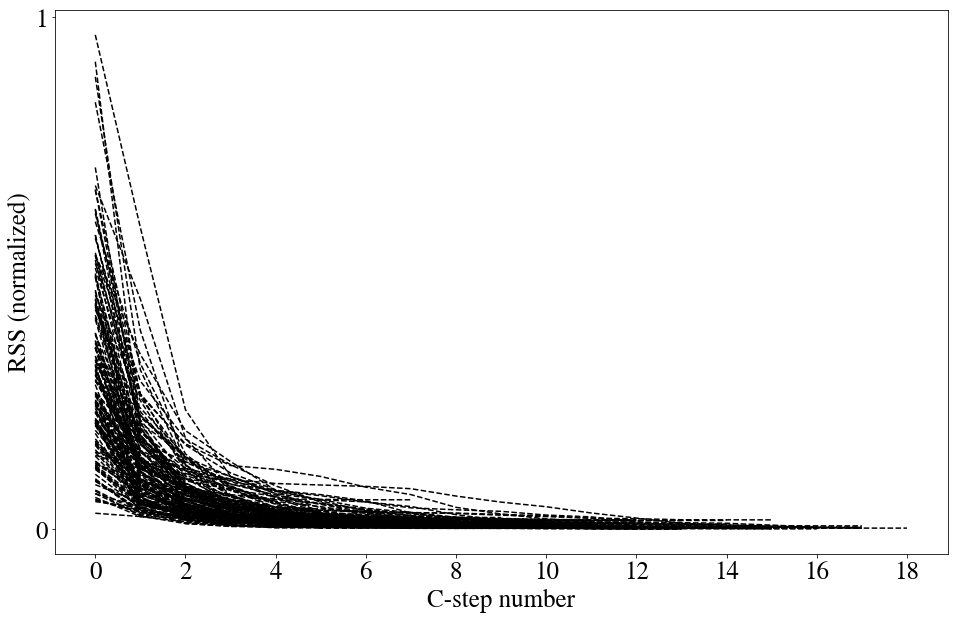
\includegraphics[width=12cm]{img/lts_convergence}
\caption{Value of the residual sum of squares (normalized) based on the number of the step of C-step algorithm for 100 different starting subsets. Dataset D3 was used with configuration $n=500, p=20$ and $30\%$ of the the outliers (see Section~\ref{chapterexperiments} for more details about the dataset). }
\label{figure:repeat:c:steps:cnt:converge}
\end{figure}

Now we can describe the final algorithm from~\cite{rouss:2000}: Choose a lot of initial subsets $\vec{m_1}$ and for each of them apply the Repeat-C-step algorithm. From all resulting subsets with the corresponding $\vec{\hat{w}}$ estimates choose the one with the least value of $\oflts(\vec{\hat{w}})$. 

Before we can construct final the algorithm, we must decide how to choose the initial subset $\vec{m_1}$ and how many of them means ``\emph{a lot}''.



%%%%%%%%      INITIAL M_1 SUBSET      %%%%%%%%%%%%%

\subsection{Choosing an initial $\vec{m_1}$ subset}

It is important to note, that when we choose $\vec{m_1}$ subset such that it contains outliers, then iteration of  C-steps usually does not converge to a good results, so we should focus on methods with non zero probability of selecting $\vec{m_1}$ such that it does not contain outliers.
There are many possibilities of how to create an initial $\vec{m_1}$ subset. Let us start with the most trivial one.


%%%%%%%%      RANDOM SELECTION         %%%%%%%%%%%%%
\subsubsection*{Random selection} \label{section:random:h:samples}
Most basic way of creating the $\vec{m_1}$ subset is simply to choose random $\vec{m_1} \in Q^{(n, h)}$. The following observation shows that it is not the best way.

\begin{observation} \label{hrandomsamples}
    % With an increasing number of data samples, thus with increasing $n$, the probability of choosing among $k$ random selections of $\vec{m_{1_1}}, \ldots ,\vec{m_{1_k}}$ the probability of selecting at least one $\vec{m_{1_i}}$ such that its corresponding data samples does not contains outliers, goes to $0$.

    Assume that the $n$-element dataset contains outliers whose number is proportional to $\epsilon / n$ with $\epsilon > 0$. Let $\vec{m_{1_1}}, \ldots ,\vec{m_{1_k}}, \vec{m_{1_i}} \in Q^{(n, h)} $ be $k$ randomly selected $h$-element subset of data. Then the probability that at least one of these $h$-element subsets does not contain an outlier tends to $0$ as $n$ goes to infinity.
\end{observation}

\begin{proof}
    It follows from observation above and the fact that $h > n/2$ that
    % Consider dataset of $n$ containing $\epsilon > 0$ relative amount of outliers. Let $h$ be chosen conservatively so that $h = [(n/2] + [(p+1)/2]$ and $k$ is the number of selections random $h$-element subsets. Then
    \begin{align*}
        P(one~random~data~sample~not~an~outliers) &= (1-\epsilon) \\
        P(one~random~h~element~subset~without~outliers) &= (1-\epsilon)^h \\
        P(one~subset~with~at~least~one~outlier) &= 1-(1-\epsilon)^h \\
        P(k~subsets~with~at~least~one~outlier~in~each) &= (1-(1-\epsilon)^h)^k \\
        P(k~subsets~with~at~least~one~subset~without~outliers) &= 1-(1-(1-\epsilon)^h)^k \\
    \end{align*}
    Because
$n \rightarrow \infty$, then    
$ (1-\epsilon)^h  \rightarrow 0 $,    
$ 1- (1-\epsilon)^h  \rightarrow 1$, 
$ (1-(1-\epsilon)^h)^k  \rightarrow 1$, and 
$1- (1-(1-\epsilon)^h)^k  \rightarrow 0 $
\end{proof}

That means that we should consider other options for selecting initial $\vec{m_1}$ subset.
Authors of the algorithm came with the following solution.


%%%%%%%%%%%     P - SELECTION %%%%%%%%%%%

\subsubsection*{P-subset selection} \label{section:random:p:samples}

Let us choose a vector $\vec{c} \in Q^{(n, p)}$ and compute the rank of the matrix $\vec{X}_{C} = \vec{C}\vec{X}$, where $C = diag(\vec{c})$. If $rank(\vec{X}_{C}) < p$ add randomly selected rows of $\vec{X}$ to $\vec{X}_{C}$ without repetition until $rank(\vec{X}_{C}) = p$. 
Next let us denote $\what{0} = \oflts(\vec{c})$. Let
$\pi: \hat{n} \rightarrow \hat{n}$ be the permutation of $\hat{n}$ such that 
$|r_{\pi(1)}(\vec{c})| \leq \ldots \leq |r_{\pi(n)}(\vec{c})|$.

 Finally, let $\vec{m_1} \in Q^{(n,h)}$ be initial $h$-element subset such that $m^{(1)}_i = 1$ for $i \in \{{\pi(1)\,, \pi(2)\,,... \pi(h)\}}$ and  $m^{(1)}_i = 0$  otherwise.
\begin{observation} \label{prandomsamples}
    % With the increasing number of data samples, the probability of choosing among $k$ random selections of $\vec{c_{1_1}}, \ldots, \vec{c_{1_k}}$ the probability of selecting at least one $\vec{c_{1_i}}$ such that its corresponding data samples do not contains outliers, goes to
    Assume that the $n$-element dataset contains outliers whose number is proportional to $\epsilon / n$ with $\epsilon > 0$. Let $\vec{c_{1_1}}, \ldots ,\vec{c_{1_k}}, \vec{c_{1_i}} \in Q^{(n, p)} $ be $k$ randomly selected $p$-element subset of data. Then the probability that at least one of these $p$-element subsets does not contain an outlier tends to

\begin{equation}
    1-(1-(1-\epsilon)^h)^k  > 0.
\end{equation}
\end{observation}

\begin{proof}
    Similarly as in previous observation.
\end{proof}

The last missing piece of the algorithm is determining the number $k$ of initial subsets $\vec{m_1}$, which maximize the probability to at least one of them leads to a sequence of estimates ending up in the global minimum. Simply put, the more, the better. So before we answer this question accurately, let us discuss some key observations about the algorithm.

%%%%%%%%%%%     SPEED-UP      %%%%%%%%%%%

\subsection{Speed-up of the algorithm}
In this section, we describe essential observations which help us to formulate the final algorithm. In two subsections we describe how to optimize the current algorithm. 

%%%%%%%%%%%     SELECTIVE ITERATION      %%%%%%%%%%%
\subsubsection*{Selective iteration}
The most computationally demanding part of one C-step is computation of the OLS fit for the subset $\vec{m_i}$ and then the calculation of $n$ absolute residuals. As we stated above, convergence is usually achieved under 20 steps. So for fast algorithm run, we would like to repeat C-step as little as possible and at the same time do not lose the performance of the algorithm. 

Since the convergence of the Repeat-C-step algorithm is very fast, it turns out that we can distinguish between starts that leads to good solutions and those which does not after few C-steps iterations. Based on empiric observation, we can distinguish good or bad solution already after two or three iterations of C-steps based on the values $\oflts(\what{3})$ and $\oflts(\what{4})$ respectively (see Figure~\ref{figure:repeat:c:steps:cnt:converge}). 

So even though authors do not specify the size of $k$ explicitly, they propose that after a few C-steps we can choose (say~10) best solutions among all $\vec{m_1}$ starting subsets and continue with iterating the C-steps only using the best solutions.
Authors refer to this process as to the \defterm{selective iteration}.

\subsubsection*{Nested extension}
C-step computation is usually very fast for small $n$. It gets slow for very high $n$, say $n > 10^3$, because we need to compute the OLS estimate for the $\vec{m_i}$ subset of size $h$ which proportional to $n$ and then calculate $n$ absolute residuals.

Authors came up with a solution they call a \defterm{nested extension}. Let $k$ be number initial subsets $\vec{m_1}$. The we can describe the nested extension as follows.

\begin{itemize}
    \item If $n$ is greater than a given limit $l$, we create subset $L$ of data $|L| = l$, and divide this subset into $s$ disjoint sets $P_1, P_2,\ldots,P_s\,, |P_i| = \frac{l}{s}\,, P_i\cap P_j  = \emptyset\,, \bigcup_{i=1}^{s} P_{i} = L$.
    \item For every $P_i$ we set the number of starts $k_{P_i} = \frac{k}{l}$. 
    \item Next in every $P_i$ we create $k_{P_i}$ number of initial $\vec{m}_{P_{i_1}}$ subsets and apply C-steps few times for each of them.
    \item Choose $10$ best results from each subsets and merge them together. We get family of sets
    $F_{merged}$ containing $10$ best $\vec{m}_{P_{i_3}}$ subsets from each $P_i$.
    \item On each subset from  $F_{merged}$ family of subsets we again apply $2$ C-steps twice and then choose $10$ best results.
    \item Finally we use these $10$ best subsets and apply Repeat-C-step algorithm.
    \item As a result we choose the best of those $10$ results.
\end{itemize} 

%%%%%%%%    PUTTING ALL TOGETHER    %%%%%%%%%%%

\subsection{Putting all together}
We have described all major parts of the algorithm FAST-LTS. One last thing we need to mention is that even though C-steps iteration usually converges under $20$ steps, it is appropriate to introduce two parameters 
$i_{max}$ and $r$ which limits the number of C-steps iterations in some rare cases when convergence is too slow. Parameter $i_{max}$ denotes the maximum number of iterations in the final Repeat-C-step iteration. Parameter $r$ denotes the threshold for the stopping criterion because of the rounding errors we use $| \oflts(\what{{i}}) - \oflts(\what{{i+1}})| \leq r$ instead of 
$\oflts(\what{{i}}) = \oflts(\what{{i+1}})$ .

% When we put all together, we get the \defterm{FAST-LTS} algorithm which is described by the following pseudocode.

% \begin{algorithm}[H]
%     \label{alg:FAST-LTS}
%     \KwIn{$\boldsymbol{X} \in \mathbb{R}^{n \times p}, \boldsymbol{y} \in \mathbb{R}^{n \times 1}, m, l, s, i_{max}, t $}
%     \KwOut{ $\vec{\hat{w}_{final}}$, $\vec{m_{final}}$ }
%     \caption{FAST-LTS}
%     \SetKw{Break}{break}
%     $\what{{final}} \gets \emptyset$\;
%     $\vec{m_{final}} \gets \emptyset$\;
%     $F_{best} \gets \emptyset$\;

%     \uIf{$n \geq l$}{
%         $F_{merged} \gets \emptyset$\;
%         % for each split
%         \For{$i \gets 0$ \textbf{to} $s$}{
%             % create xx number of starts
%             $F_{selected}  \gets \emptyset$\;
%             \For{$j \gets 0$ \textbf{to} $\frac{l}{s}$}{
%               $F_{initial} \gets Selective~iteration(\frac{m}{l})$\;
%               % on each starts iterate few c steps
%               \For{$\vec{m_i}$ \textbf{in} $F_{initial}$}{
%                 $\vec{m_i} \gets Iterate~C~step~few~times(\vec{m_i})$\;
%                 $F_{selected} \gets  F_{selected} \cup \{{ \vec{m_i} \}} $\;
%               }
%             }
%             % among all starts select 10 best and add it to merged set
%             $F_{merged} \gets F_{merged} \cup Select~10~best~subsets~from~F_{selected}$\;
%           }
        
%           % for each, say 50 best, iterate few and add it to best
%           \For{$\vec{m_i}$ \textbf{in} $F_{merged}$}{
%             $\vec{m_i} \gets Iterate~C~step~few~times(\vec{m_i})$\;
%             $F_{best} \gets F_{best} \cup \{{ \vec{m_i} \}} $\;
%           }
%           $F_{best} \gets  Select~10~best~subsets~from~F_{best} $\;
%     }
%     \Else{
%         $F_{initial} \gets Selective~iteration(m)$\;
%         $F_{best} \gets  Select~10~best~subsets~from~F_{initial} $\;
%     }

%     % iterate till convergence on few best final results
%     $F_{final} \gets \emptyset$\;
%     $W_{final} \gets \emptyset$\;
%     \For{$\vec{m_i}$ \textbf{in} $F_{best}$}{
%             $\vec{m_i}, \what{i} \gets Iterate~C~step~till~convergence(\vec{m_i}, i_{max}, t)$\;
%             $F_{final} \gets F_{final} \cup \{{ \vec{m_i} \}}$\;
%             $W_{final} \gets W_{final} \cup \{{ \what{i} \}}$\;
%     }

%     % select one best result
%     $\what{{final}}, \vec{m_{final}} \gets select~\vec{\hat{w_i}}~and~\vec{m_{i}}~with~smallest~\oflts(\vec{\hat{w_i}})~from~F_{final}$\;

%     \Return{ $\what{{final}}, \vec{m_{final}}$  }\;
% \end{algorithm}






%%%%%%%%%%%%%%%%%%%%%%%%%%%%%%%%%%
%%%%%%%        FEASIBLE SOLUTION        %%%%%%%%%%%%
%%%%%%%%%%%%%%%%%%%%%%%%%%%%%%%%%%

\section{Feasible solution} \label{section_feasible_solution}
In this section we introduce feasible solution algorithm from~\cite{hawkins:1994}.
It is based on the strong necessary condition described at Definition~\ref{strong_condition}. 
The basic idea can be described as follows.

Let us consider that we have some $\vec{m} \in Q^{(n,h)}$, then we can denote $O_m = \{{i \in  \set{ 1,2,\ldots , n } ;w_i = 1\}}$ and $Z_m = \{{j \in  \set{ 1,2,\ldots , n } ;w_j = 0\}}$ thus sets of indexes of positions where is $0$ respectively $1$ in vector $\vec{m}$. We can think about it as indexes of observations in $h$ set and $g$ set respectively. Then we can mark $\vec{m}^{(i,j)}$ as a vector which is constructed by swap of its ith and jth element where $i \in O$ and $j \in Z$. Such vector corresponds to vector $\vec{m_{swap}}$ which we marked at Definition~\ref{strong_condition}.

With this in mind, let us mark 
\begin{equation}
    \Delta S^{(\vec{m})}_{i,j} = \oflts(\vec{m}^{(i,j)}) - \oflts(\vec{m})
\end{equation}
thus a change of the LTS objective function by swapping one observation from not trimmed subset with another from trimmed subset. To calculate this we can obviously first calculate the  $\oflts(\vec{m})$ and  the $ \oflts(\vec{m}^{(i,j)})$ and finally subtract both results. Although it is a option, it it computationally exhaustive. So the question is if there is easier way of calculating $\Delta S^{(\vec{m})}_{i,j}$. The answer is positive and we describe it now.

Let us mark  
$M = diag(\vec{m})$ and 
$M^{(i,j)} = diag(\vec{m}^{(i,j)})$ and also
$\vec{Z_M} = (\vec{X}^T\vec{M}^T\vec{X})$
For now let us assume that we also have
$\vec{Z_M}^{-1}$ and $\vec{\hat{w}} = \vec{Z_M}^{-1}\vec{X}^T\vec{M}\vec{y}$.
We now want to calculate $\Delta S^{(\vec{m})}_{i,j}$.
Let us mark vector of residuals 
$\vec{r}^{(\vec{m})} = \vec{Y} - \vec{X} \vec{\hat{w}} $
and also $d_{r,s} = \vec{x_r} \vec{Z_M}^{-1}  \vec{x_s} $
then by equation introduced in~\cite{atkinson1991simulated} we get

\begin{equation} \label{hawkins:rovnice}
    \Delta S^{(\vec{m})}_{i,j} = 
    \frac{({r}^{(\vec{m})}_{j})^2(1-d_{i,i})- ({r}^{(\vec{m})}_{i})^2(1+d_{j,j}) + 2{r}^{(\vec{m})}_{i}{r}^{(\vec{m})}_{j}d_{j,j}}
    {(1-d_{i,i})(1+d_{j,j}) + d_{i,j}^2}.
\end{equation}

Let us now describe the core of the algorithm. It is similar to the FAST-LTS algorithm in the sense of iterative refinement of a $h$-element subset. So let us assume that we have some vector  $\vec{m} \in Q^{(n,h)}$. No we compute  $\Delta S^{(\vec{m})}_{i,j}$ for all $i \in O$ and $j \in Z$. This may lead to several different outcomes:
\begin{enumerate}
    \item all $S^{(\vec{m})}_{i,j}$ are non-negative
    \item one $S^{(\vec{m})}_{i,j}$ is negative
    \item multiple $S^{(\vec{m})}_{i,j}$ are negative
\end{enumerate}

In the first case, all $\oflts(\vec{m}^{(i,j)})$ are higher or the same as the $\oflts(\vec{m})$ so none swap will lead to an improvement. That also means that strong necessary condition is satisfied and the algorithm ends.

In the second and third case, the strong necessary condition is not satisfied, and we can make the swap. In the second case, it is easy which one to choose because we have only one. In the third case, we have a couple of options again:
\begin{enumerate}
    \item use the first swap that leads to the improvement
    \item from all possible swaps choose one that has highest improvement value  $\oflts(\vec{m}^{(i,j)})$
    \item use the first swap that has improvement higher than some given threshold
\end{enumerate}

In terms of complexity, all three options give the same results, because to find a feasible solution you need to evaluate all pair swaps. In practice, the third option is the winner because it leads to the least amount of iterations. On the other hand, as we said this does not improve the complexity of the algorithm, so from now on let us assume that we use the case number two.
So if there negative  $S^{(\vec{m})}_{i,j}$, we choose the one with the lowest value, make the swap and repeat the process.  

The algorithm ends when there is no possible improvement, i.e., when all $S^{(\vec{m})}_{i,j}$ are non-negative.
The number of iterations needed till algorithm stops is usually quite low, but for practical usage, it is still convenient to use some parameter $i_{max}$ after which algorithm stops without finding $h$-element subset satisfying the strong necessary condition. 
One step of this algorithm we call optimal swap additive algorithm (OSAA) is described by the following pseudocode.

\begin{algorithm}[H]
    \label{alg:optimal:improvement}
    \KwIn{$\vec{Z_M}^{-1} \in \mathbb{R}^{p \times p}$, 
    $\vec{r}^{(\vec{m})} \in \mathbb{R}^{n \times 1}$, 
    $O_m$, $Z_m$, $\vec{X} \in \mathbb{R}^{n \times p} $}
    \KwOut{ $\what{{new}}$, $m_{new}$ }
    \caption{OSAA}
    
    $S \gets 0$\;
    $i_{swap} \gets \emptyset$\;
    $j_{swap} \gets \emptyset$\;

    \For{$m_i \in  O_m$}{  
        \For{$m_j \in  Z_m$}{ 
            $r_i^{(m)} = \vec{r}^{(\vec{m})}_{m_i}$ \;
            $r_j^{(m)} = \vec{r}^{(\vec{m})}_{m_j}$ \;
            $d_{i,i} = \vec{x_{m_i}} \vec{Z_M}^{-1} \vec{x^T_{m_i}}$ \;
            $d_{i,j} = \vec{x_{m_i}} \vec{Z_M}^{-1} \vec{x^T_{m_j}}$ \;
            $d_{j,j} = \vec{x_{m_j}} \vec{Z_M}^{-1} \vec{x^T_{m_j}}$ \;
            $S_{tmp} = calculate~\Delta S^{(\vec{m})}_{i,j}~by$ \eqref{hawkins:rovnice} \;
            \If{$S_{tmp} < S$}{
                $S \gets S_{tmp}$\;
                $i_{swap} \gets m_i$\;
                $j_{swap} \gets m_j$\;
            }
        }
    }
    \Return{ $i_{swap}, j_{swap}, S$ }\;
\end{algorithm}


\begin{observation} 
     The time complexity of the OSAA~\ref{alg:optimal:improvement} is $\mathcal{O}(n^2p^2)$
\end{observation} 


\begin{proof}
All $d_{i,i}$ and $d_{j,j}$ can be calculated before the for loops. 
To calculate $d_{i,i}$ resp. $d_{j,j}$ we need co multiply vector $\in \mathbb{R}^p$ with matrix  $\in \mathbb{R}^{p \times p}$ and vector $\in \mathbb{R}^p$ that is $\mathcal{O}(p^2)$. For all $d_{i,i}$ this have to be done $h$ times and for $d_{j,j}$ $n-h$ times. So all together it is $\mathcal{O}(np^2)$. 

The two loops go through all pairs; thus it is $\mathcal{O}(n^2)$. $d_{i,j}$ can be calculated in the loop, and it can be done in $\mathcal{O}(p^2)$.

If we put everything together we get 
$\mathcal{O}(np^2 + n^2p^2) \sim \mathcal{O}(n^2p^2)$.
\end{proof}


One run of this iteration process leads to some local optimum, i.e., set satisfying the strong necessary condition. In~\cite{hawkins:1994} they refer to to this set as to \defterm{feasible set}.
This because it is not global optima the algorithm needs to be run multiple times say $t$ times. A $h$  subset with the smallest value of the objective function is chosen as the final solution.

Discussion about how to find the initial $h$-element subset resp. initial $\vec{m}$ was already discussed when describing FAST-LTS algorithm.
More importantly, as we already suggested $h$-element subset satisfying weak necessary condition do not need to satisfy strong necessary condition so passing such a $h$-element subset as input to this algorithm is another option and we discuss it in detail later. We now describe a feasible solution algorithm (FSA) with pseudocode, and we assume that we already have some function that generates for us $h$-element subsets, e.g., random one. 

\newcommand\mycommfont[1]{\footnotesize\ttfamily\textcolor{blue}{#1}}
\SetCommentSty{mycommfont}

\begin{algorithm}[H]
    \label{alg:feasible_solution}
        \KwIn{$\boldsymbol{X} \in \mathbb{R}^{n \times p}, \boldsymbol{y} \in \mathbb{R}^{n \times 1},  i_{max}, t $}
        \KwOut{ $\vec{\hat{w}_{final}}$, $\vec{m_{final}}$ }
        
    \caption{FSA}
    \SetKw{Break}{break}
    $\vec{\hat{w}_{final}} \gets \emptyset$\;
    $\vec{m_{final}} \gets \emptyset$\;
    $R \gets \emptyset$\;

    \For{$k \gets 0$ \textbf{to} $t$}{
        $\vec{m} \gets generate\_intial\_subset()$  \tcp*{e.g. random $\vec{m} \in Q^{(n,h)}$}

    $l \gets 0$\;
        \While{$True$}{           
           $\vec{M} \gets diag(\vec{m})$\;
       $\vec{Z_M} = (\vec{X}^T\vec{M}^T\vec{X})$\;
       $\vec{Z_M}^{-1} = calculate~inversion~of~\vec{Z_M}$\;
       $\vec{\hat{w}} \gets \of^{(OLS,\vec{M}\vec{X},  \vec{M}\vec{y} )}$\;
       $\vec{r}^{(\vec{m})} = \vec{Y} - \vec{X} \vec{\hat{w}}$\;
      
    $S_{i,j}, i, j$ = 
       $OSAA$(
            $\vec{Z_M}^{-1}$, 
                $\vec{r}^{(\vec{m})}$, 
                $O_m$, 
                        $Z_m$, 
                        $\vec{X}$)\;

            \If{$ S_{i,j} \geq 0$ \textbf{or}  $l \geq i_{max}$ }{
                $\vec{m_{final}} \gets \vec{m}$\;
                $\vec{\hat{w}} \gets \of^{(OLS,\vec{M}\vec{X},  \vec{M}\vec{y} )}$\;
                $R \gets R \cup \{\vec{m_{final}} , \vec{\hat{w}} \}$\;
                \Break\;
            }
            \Else {
                $\vec{m} \gets \vec{m}^{(i,j)}$\;
            }
        }        
    }
    $\vec{m_{final}}, \vec{\hat{w}_{final}}  \gets $ select best from $R$ based on smallest value of $\oflts$\;
    \Return{ $\what{{final}}$\,, $\vec{m_{final}}$ }\;
\end{algorithm}



\begin{observation}  \label{time:complexity:fsa}
In the main loop beside running OSAA which time complexity is $\mathcal{O}(n^2p^2)$ we need to recalculate $\vec{\hat{w}}$ using the matrix inversion which time complexity is $\mathcal{O}(p^2n)$ (see Observation~\ref{time:complexity:ols:inversion}).
Main loop of the FSA runs up to $l$ iterations for each start $t$. So the time complexity of whole algorithm is  $\mathcal{O}( lt(n^2p^2 + p^2n)  )$. Because $l$ and $t$ are usually quite low, we can see that the FSA time complexity is dominated by the OSAA. 
\end{observation} 

In this section, we've described the FSA algorithm. In the next section, we introduce a very similar algorithm, but which have higher numerical stability and also contains various optimizations for higher performance.







%%%%%%%%%%%%%%%%%%%%%%%%%%%%%%%%%%%%
%%%%% OEA, MOEA, MMEA %%%%%%%%%%%%%%
%%%%%%%%%%%%%%%%%%%%%%%%%%%%%%%%%%%%

\section{OEA, MOEA, MMEA} \label{oeamoeammea}
%three exchanging algorithms from Agulló, 2000

In the FSA algorithm, we assumed that after each cycle of OSAA~\ref{alg:optimal:improvement} we need to recalculate inversion $(\vec{X}^T\vec{X})$ together with $\vec{\hat{w}}$. In this section, we introduce a different approach described in~\cite{agullo2001new} so that we can update it instead of recalculating. Moreover, these ideas lead to bounding condition of FSA which not only improves the speed but also gives options to construct different algorithms. 

In Section~\ref{section_feasible_solution} we introduce additive formula~\eqref{hawkins:rovnice} which corresponds to $\oflts(\vec{m}^{(i,j)}) - \oflts(\vec{m})$. Let us now try to obtain similar formula but with the focus on how the individual elements in our current algorithm change namely the inversion $\vec{Z^{-1}}$ and $\vec{\hat{w}}$. We also split the idea of swap the $i, j$ into the insertion of $j$ and remove of $i$. Thus we describe how individual elements are affected after adding one row and also removing one row. Moreover, during this derivation, we obtain two different approaches to calculate it. Both are important, and we recapitulate them after.




%%%%%%% MULTIPLICATIVE INCREMENT FORMULA   %%%%%%%%%

\subsection{Multiplicative formula}



$\vec{Z} = \vec{X}^T\vec{X}$
Let us denote $\vec{A} = (\vec{X}, \vec{y})$, a matrix $\vec{X}$ expanded by one column of corresponding dependent variables and and $\vec{\tilde{Z}} = \vec{A}^T\vec{A}$. Then

\[  \numberthis \label{matrixZ}
    \vec{\tilde{Z}} = \begin{bmatrix}
        \vec{Z} & \vec{X}^T\vec{y} \\
    \vec{y}^T\vec{X} & \vec{y}^T\vec{y}
  \end{bmatrix} .
\]
Notice that $\vec{Z}$ is symmetric square matrix $\in \mathbb{R}^ {p \times p}$, moreover we suppose that $Z$ is regular. $\vec{X}^T\vec{y}$ is $p$ dimensional column vector, $\vec{y}^T\vec{X}$ is $p$ dimensional row vector and $\vec{y}^T\vec{y}$ is a scalar.
OLS estimate $\vec{\hat{w}}$ is then given by
\begin{equation}
    \vec{\hat{w}}^{(OLS,\vec{X}, \vec{y})} = \vec{Z}^{-1} \vec{X}^T\vec{y}
\end{equation}
and the RSS by 

\begin{equation}
    RSS = \vec{y}^T\vec{y} - \vec{y}^T\vec{X}\vec{\hat{w}}.
\end{equation}
Also, note that all necessary matrix multiplications are already in the matrix $\vec{\tilde{Z}}$.

Let us show that $RSS$ can  be expressed as ratio of determinants $\det(\vec{\tilde{Z}})$ and $\det(\vec{Z})$ (using determinant rule for block matrices) so that 

\begin{align*} \numberthis \label{rssdeterminant} 
    RSS &= \frac{\det(\vec{\tilde{Z}})}{\det(\vec{Z})} \\ &= \frac{
    \det\begin{pmatrix}
            \vec{Z} & \vec{X}^T\vec{y} \\
            \vec{y}^T\vec{X} & \vec{y}^T\vec{y}
        \end{pmatrix}
        }{\det\left(\vec{M}\right)}\\
         &=\frac{ \det(\vec{Z}) \det\left(\vec{y}^T\vec{y} -  \vec{y}^T\vec{X} \vec{Z}^{-1} \vec{y}\right) }
        {\det\left(\vec{Z}\right)} \\ 
        &= \vec{y}^T\vec{y} - \vec{y}^T\vec{X}\vec{\hat{w}}.
\end{align*}

If we assume that $RSS > 0$ then $\vec{\tilde{Z}}^{-1}$ can be expressed as 

\[ \numberthis
    \vec{\tilde{Z}}^{-1} = 
    \begin{bmatrix}
        \vec{Z}^{-1}+\dfrac{\vec{\hat{w}} \vec{\hat{w}}}{RSS} & - \dfrac{\vec{\hat{w}}^T}{RSS} \\[6pt]
        - \dfrac{\vec{\hat{w}^{T}}}{RSS} & \dfrac{1}{RSS}
    \end{bmatrix}.
\]
For following equations it is important to notice that for any two row vectors $\vec{c_i} = (\vec{x_i}, y_i)$  and $\vec{c_j} = (\vec{x_j}, y_j)$, $\vec{c_i}, \vec{c_j} \in \mathbb{R}^{1 \times p+1}$ is 

\begin{equation}
    \vec{c_i} \vec{\tilde{Z}}^{-1} \vec{c_i^T} = \dfrac{ ( y_i - \vec{x_i}\vec{\hat{w}} )^2 }{RSS}  + \vec{x_i}\vec{Z}^{-1}\vec{x_i^T}
\end{equation}
and
\begin{equation}
    \vec{c_j} \vec{\tilde{Z}}^{-1} \vec{c_j^T} = \dfrac{ ( y_j - \vec{x_j}\vec{\hat{w}} ) ( y_i - \vec{x_i}\vec{\hat{w}} ) }{RSS}  + \vec{x_j}\vec{Z}^{-1}\vec{x_j^T}
\end{equation}



%%%%%%% INCLUDING OBSERVATION %%%%%%%%%%%

\subsubsection*{Including the observation} 

Using above let us express how the determinant $\det(\vec{Z})$ and the inverse of the $vec{Z}^{-1}$ changes when observation $\vec{c_i} = (\vec{x_i}, y_i)$ is added to the matrix $\vec{A}$. First let us notice that if we add this row to $\vec{A}$, then  $\vec{Z}$ changes as

\[ \numberthis \label{addedrow}
\begin{bmatrix}
    x_{11} & x_{12} & \dots  & x_{1n} & x_{i_1}  \\
    x_{21} & x_{22} & \dots  & x_{2n} & x_{i_2} \\
    \vdots & \vdots & \vdots & \ddots & \vdots \\
    x_{p1} & x_{p2} & \dots  & x_{pn} & x_{i_p}     
\end{bmatrix}
\begin{bmatrix}
    x_{11} & x_{12}  & \dots  & x_{1p} \\
    x_{21} & x_{22}  & \dots  & x_{2p} \\
    \vdots  & \vdots & \ddots & \vdots \\
    x_{n1} & x_{n2}  & \dots  & x_{np} \\
    x_{i_1} & x_{i_2}  & \dots  & x_{i_p}
\end{bmatrix}
 = \vec{X}^T\vec{X} + \vec{x_i^T}\vec{x_i} = \vec{Z} + \vec{x_i^T}\vec{x_i},
\]
so determinant with appended row changes as
\begin{equation} \label{udpateddeterminant}
    \det(\vec{Z} + \vec{x_i^T}\vec{x_i}) = det(\vec{Z})(1 + \vec{x_i}\vec{Z}^{-1}\vec{x_i^T}).
\end{equation}
Finally the inversion $\vec{Z}^{-1}$ can be obtained using Sherman-Morrison formula~\cite{bartlett1951inverse} so that 
\begin{equation} \label{shermanmorris}
    (\vec{Z} + \vec{x_i^T}\vec{x_i})^{-1} = \vec{Z}^{-1} - \dfrac{\vec{Z}^{-1}\vec{x_i^T}\vec{x_i}\vec{Z}^{-1}}{1 + \vec{x_i}\vec{Z}^{-1}\vec{x_i^T}}
\end{equation}

It is now convenient to denote 
\begin{equation}
    b = \dfrac{-1}{(1 + \vec{x_i}\vec{Z}^{-1}\vec{x_i^T})},  b \in \mathbb{R},
\end{equation}
and 
\begin{equation} \label{agullo_u}
    \vec{u} = \vec{Z}^{-1}\vec{x_i^T},      \vec{u} \in \mathbb{R}^{p \times 1}.
\end{equation}

Then~\eqref{shermanmorris} can be written as
\begin{equation} \label{inversionplus}
    (\vec{Z} + \vec{x_i^T}\vec{x_i})^{-1} = \vec{Z}^{-1} + b\vec{u}\vec{u^T}.
\end{equation}

Given that last missing piece to express updated $\vec{\hat{w}}$ is appended $\vec{X}^T\vec{y}$ by one row, which can be simply expressed by same idea as~\eqref{addedrow} so that updated $\vec{\hat{w}}$ which we denote as $\vec{\overline{\hat{w}}}$ is 
\begin{equation}
    \vec{\overline{\hat{w}}} = (\vec{Z}^{-1} + b\vec{u}\vec{u^T})(\vec{X^T}\vec{y} + y_i\vec{x_i^T}).
\end{equation}
This can be simplified so that we get
\todo{mention the mistake in original paper? w + (y - xw)bu ??}
\begin{equation} \label{thetaplus}
    \vec{\overline{\hat{w}}} = \vec{\hat{w}} - (y_i - \vec{x_i}\vec{\hat{w}})b\vec{u}.
\end{equation}
Least but not last we want to express updated $RSS$ which we denote as $\overline{RSS}$. This can be done easily from~\eqref{rssdeterminant} and~\eqref{udpateddeterminant} as 

\begin{equation}
    \overline{RSS} =  RSS + \dfrac{(y_i - \vec{x_i}\vec{\hat{w})^2}}{(1 + \vec{x_i}\vec{Z}^{-1}\vec{x_i^T})}.
\end{equation}
It is convenient to mark 
\begin{equation} \label{gamma:plus}
    \gamma^{+}(\vec{c_i}) = \dfrac{(y_i - \vec{x_i}\vec{\hat{w})^2}}{(1 + \vec{x_i}\vec{Z}^{-1}\vec{x_i^T})},
\end{equation}
so that 
\begin{equation} \label{rssplus}
    \overline{RSS} =  RSS + \gamma^{+}(\vec{c_i})
\end{equation}
We can see that $\gamma^{+}(\vec{c_i})$ measures how $RSS$ increase after we append our dataset with observation $\vec{c_i}$, thus $\gamma^{+}(\vec{c_i}) \geq 0$



%%%%%%% EXCLUDING OBSERVATION %%%%%%%%%%%

\subsubsection*{Excluding the observation}

Because we want to express both increment and decrement change in our dataset, let us now focus how $RSS$, $\vec{Z^{-1}}$ and $\vec{\hat{w}}$  changes after we exclude one observation. 

Consider that we already included one observation $\vec{c_i}$ in our dataset and mark $\vec{\overline{Z}} = \vec{Z} + \vec{x_i} \vec{x_i^T} $. If we exclude one observation $\vec{c_j} = (\vec{x_j}, y_j) \in \mathbb{R}^{p+1 \times 1} $ from already updated matrix $\vec{A}$ then the determinant $\det(\vec{\overline{Z}})$  changes as

\begin{equation} 
    \det(\vec{\overline{Z}} - \vec{x_j^T}\vec{x_j}) = det(\vec{\overline{Z}})(1 - \vec{x_j}\vec{\overline{Z}}^{-1}\vec{x_j^T})
\end{equation}
and the inversion changes (again, according to Sherman-Morrison formula) as 
\begin{equation}  
    (\vec{\overline{Z}} - \vec{x_j^T}\vec{x_j})^{-1} = \vec{\overline{Z}}^{-1} + \dfrac{\vec{\overline{Z}}^{-1}\vec{x_j^T}\vec{x_j}\vec{\overline{Z}}^{-1}}{1 - \vec{x_j}\vec{\overline{Z}}^{-1}\vec{x_j^T}}.
\end{equation}

Once again, it is convenient to denote
\begin{equation}
    \overline{b} = \dfrac{-1}{(1  \vec{x_j}\vec{\overline{Z}}^{-1}\vec{x_j^T})},  \overline{b} \in \mathbb{R},
\end{equation}
and 
\begin{equation}
    \vec{\overline{u}} = \vec{\overline{Z}}^{-1}\vec{x_j^T},      \vec{\overline{u}} \in \mathbb{R}^{p \times 1},
\end{equation}
so that we can write
\begin{equation} \label{updatedinversion2}
    (\vec{\overline{Z}} + \vec{x_j^T}\vec{x_j})^{-1} = \vec{Z}^{-1} - \overline{b}\vec{\overline{u}}\vec{\overline{u}^T}.
\end{equation}

Using the same approach as before we can denote express down-dated estimate which we denote as $\vec{\overline{\overline{\hat{w}}}}$

\begin{equation} \label{thetaminus}
    \vec{\overline{\overline{\hat{w}}}} =  +\vec{\overline{\hat{w}}} (y_j - \vec{x_j}\vec{\overline{\hat{w}}}) \overline{b} \vec{\overline{u}}.
\end{equation}

Finally lets also express updated $\overline{RSS}$ which we denote as $\overline{\overline{RSS}}$. This can be done easily from~\eqref{rssdeterminant} and~\eqref{udpateddeterminant} and~\eqref{updatedinversion2} as 

\begin{equation}
    \overline{\overline{RSS}} =  \overline{RSS} - \dfrac{(y_j - \vec{x_j}\vec{\overline{\hat{w}})^2}}{(1 - \vec{x_j}\vec{\overline{{Z}}}^{-1}\vec{x_j^T})}.
\end{equation}

Let us mark

\begin{equation} \label{gamma:minus}
    \gamma^{-}(\vec{c_j}) = \dfrac{(y_j - \vec{x_j}\vec{\overline{\hat{w}})^2}}{(1 - \vec{x_j}\vec{\overline{{Z}}}^{-1}\vec{x_j^T})},
\end{equation}
so that 
\begin{equation} \label{rssminus}
    \overline{\overline{RSS}} =  \overline{RSS} - \gamma^{-}(\vec{c_j}).
\end{equation}



%%%%%%      S W A P P I N G    T W O   O B S E R V A T I O N S     %%%%%

\subsubsection*{Swapping two observations}

Let us now express the equation for including and excluding observation at once. First, notice that from~\eqref{updatedinversion2} we can express 

\begin{equation} \label{xjoverlinez}
    \vec{x_j}\vec{\overline{{Z}}}^{-1}\vec{x_j^T}) =  \vec{x_j}\vec{Z}^{-1}\vec{x_j^T}) - 
    \dfrac{( \vec{x_i}\vec{Z}^{-1}\vec{x_j^T})^2}{1 +  \vec{x_i}\vec{Z}^{-1}\vec{x_i^T})},
\end{equation}
 so that 

 \begin{gather}
 \begin{align*} \numberthis
    &\det(\vec{Z} + \vec{x_i^T}\vec{x_i} - \vec{x_j^T}\vec{x_j}) = \\
    \det(\vec{Z})(1 + \vec{x_i}\vec{Z}^{-1}\vec{x_i^T} -& \vec{x_j}\vec{Z}^{-1}\vec{x_j^T} +  ( \vec{x_i}\vec{Z}^{-1}\vec{x_j^T})^2 - \vec{x_i}\vec{Z}^{-1}\vec{x_i^T}\vec{x_j}\vec{Z}^{-1}\vec{x_j^T} )
\end{align*}
\end{gather}

Finally we can express the $\overline{\overline{RSS}} $ as

\begin{equation} \label{updaterss}
    \overline{\overline{RSS}}  = RSS\rho(\vec{c_i}, \vec{c_j}),
\end{equation}
where
\begin{equation} \label{agullo:rovnice}
    \rho(\vec{c_i}, \vec{c_j}) =
     \dfrac
     {(1+\vec{x_i}\vec{Z}^{-1}\vec{x_i^T} + \dfrac{e_j^2}{RSS})
        (1 - \vec{x_j}\vec{Z}^{-1}\vec{x_j^T} - \dfrac{e_i^2}{RSS} )+
        (\vec{x_i}\vec{Z}^{-1}\vec{x_j^T} + \dfrac{e_i e_j}{RSS} )^2}
    {1 + \vec{x_i}\vec{Z}^{-1}\vec{x_i^T}  - \vec{x_j}\vec{Z}^{-1}\vec{x_j^T}  + ( \vec{x_i}\vec{Z}^{-1}\vec{x_j^T})^2 -   \vec{x_i}\vec{Z}^{-1}\vec{x_i^T}\vec{x_j}\vec{Z}^{-1}\vec{x_j^T} },
\end{equation}
where $e_i = y_i - x_i\vec{\hat{w}}$ and $e_j = y_j - x_j\vec{\hat{w}}$.

We can see that this formula is similar to the~\eqref{hawkins:rovnice} but here the $\rho(\vec{c_i}, \vec{c_j})$ represents multiplicative increment. Moreover $0 < \rho(\vec{c_i}, \vec{c_j}) $ and if $0 < \rho(\vec{c_i}, \vec{c_j})< 1$ then the swap leads to improvement in terms of feasible solution.

We are now able to modify the FSA so that we do not need to recompute $\vec{\hat{w}}$ and inversion $(\vec{X}^T \vec{X})^{-1}$ but we can update it. Authors call this algorithm optimal exchange algorithm (OEA)





%%%%%%%%%%%%%%%%%%%%%%%%%%%%%%%%%%%%%%%
%%%%%%%%%%     O E A    A L G O R I TH M        %%%%%%%%%%%%%

\subsection{The OEA and its properties}
We can apply theory from the previous section to the FSA. Sets $O_m$ and $Z_m$ (see Section~\ref{section_feasible_solution}) contains indexes of observations to exclude and include respectively.
The matrix $\vec{Z_M}$ can be used instead of the matrix $\vec{Z}$ and
 $\vec{X_M}$ with $\vec{y_M}$ to calculate $\vec{\hat{w}}$. 

In terms of the FSA~\ref{alg:feasible_solution} we first need to change the OSAA.  There are only minor tweaks. First, we need to pass one more argument, and that is $RSS$. Second, We want to find minimal $\rho(\vec{c_i}, \vec{c_j})$ calculated by~\eqref{agullo:rovnice} so that $0 < \rho(\vec{c_i}, \vec{c_j}) < 1 $. Other parts of the algorithm remains the same. Time complexity thus remains the same.

This algorithm produces $\rho(\vec{c_i}$, and indexes  $i_{swap} \in O_m$ and $j_{swap} \in Z_m$ of observations we want to swap. Given that, we can update the $RSS$ by~\eqref{updaterss}, $\vec{Z_M^{-1}}$ by~\eqref{inversionplus} and~\eqref{updatedinversion2} and finally update $\vec{\hat{w}}$ by~\eqref{thetaplus} and~\eqref{thetaminus}.

Let us now talk about the time complexity of such a solution. As we said, the time complexity of modifies OSAA is $\mathcal{O}( n^2 p^2)$. Thus there is no asymptotic improvement. On the other hand, there are some significant constants outside the OSAA so let us look at how they improve.

When an improvement is found, thus when $0 < \rho(\vec{c_i}, \vec{c_j}) < 1 $, then we update $RSS$, which is constant. Next we update inversion by~\eqref{inversionplus} which is $\mathcal{O}(4p^2)$ and~\eqref{updatedinversion2} which is also $\mathcal{O}(4p^2)$.  Finally we need to update $\vec{\hat{w}}$ by~\eqref{thetaplus} and~\eqref{thetaminus} which are both $\mathcal{O}(p^2 +p)$. 

\begin{observation} \label{updatinginversionobservation}
Time complexity of updating all the quantities is 
$\mathcal{O}(8p^2 + 2p^2 + p) \sim \mathcal{O}(p^2)$.
That is quite an improvement if we compare it to time complexity $\mathcal{O}(p^2n)$ of updating those quantities in the FSA (see Observation~\ref{time:complexity:fsa}).
\end{observation}


Note that right now it actually does not matter if we use additive formula~\eqref{hawkins:rovnice} with the stopping criterion $\Delta S^{(\vec{m})}_{i,j} \geq 0$ --- thus unmodified OSAA --- or multiplicative formula~\eqref{agullo:rovnice} with the stopping criterion $\rho(\vec{c_i}, \vec{c_j}) \geq 1 $. Both results we can update $RSS$ and other quantities can be used to calculate both formulas. 

However, the advantage of the multiplicative formula~\eqref{agullo:rovnice} is that we can use the following bounding condition to improve the performance of the modified OSAA.


%%%%%       B O U N D I N G   C O N D I T I ON    S P E E D U P       %%%%%

\subsubsection*{Bounding condition improvement}

The $\rho(\vec{c_i}, \vec{c_j})$ is expressed as a ratio. We can see that in the numerator we have

\begin{equation}
    (1+\vec{x_i}\vec{Z}^{-1}\vec{x_i^T} + \dfrac{e_j^2}{RSS})
        (1 - \vec{x_j}\vec{Z}^{-1}\vec{x_j^T} - \dfrac{e_i^2}{RSS} )+
        (\vec{x_i}\vec{Z}^{-1}\vec{x_j^T} + \dfrac{e_i e_j}{RSS} )^2,
\end{equation}
and because $ \dfrac{e_i e_j}{RSS} )^2 \geq 0$ then whole numerator is greater or equal to
\begin{equation}
    (1+\vec{x_i}\vec{Z}^{-1}\vec{x_i^T} + \dfrac{e_j^2}{RSS})
(1 - \vec{x_j}\vec{Z}^{-1}\vec{x_j^T} - \dfrac{e_i^2}{RSS} ).
\end{equation}
On the other hand, we can see that denominator is

\begin{equation}
    1 + \vec{x_i}\vec{Z}^{-1}\vec{x_i^T}  - \vec{x_j}\vec{Z}^{-1}\vec{x_j^T}  + (\vec{x_i}\vec{Z}^{-1}\vec{x_j^T})^2 -   \vec{x_i}\vec{Z}^{-1}\vec{x_i^T}\vec{x_j}\vec{Z}^{-1}\vec{x_j^T}, 
\end{equation}
and because $(\vec{x_i}\vec{Z}^{-1}\vec{x_j^T})^2$ and $\vec{x_i}\vec{Z}^{-1}\vec{x_i^T}\vec{x_j}\vec{Z}^{-1}\vec{x_j^T} $ are actually inner products of $\vec{x_i}$ and $\vec{x_j}$  ($\vec{Z}^{-1}$ is positive definite) thus
\begin{equation}
    (\vec{x_i}\vec{Z}^{-1}\vec{x_j^T})^2 \leq \vec{x_i}\vec{Z}^{-1}\vec{x_i^T}\vec{x_j}
\end{equation}
using the Cauchy-Schwarz inequality. This means that denominator is less or equal to
\begin{equation}
    1 + \vec{x_i}\vec{Z}^{-1}\vec{x_i^T}  - \vec{x_j}\vec{Z}^{-1}\vec{x_j^T}.
\end{equation}
Given that we can denote $\rho_b(\vec{c_i}, \vec{c_j})$  as

\begin{equation} \label{boundingcondition}
\rho_b(\vec{c_i}, \vec{c_j}) = \dfrac{(1+\vec{x_i}\vec{Z}^{-1}\vec{x_i^T} + \dfrac{e_j^2}{RSS})
    (1 - \vec{x_j}\vec{Z}^{-1}\vec{x_j^T} - \dfrac{e_i^2}{RSS} )}{1 + \vec{x_i}\vec{Z}^{-1}\vec{x_i^T}  - \vec{x_j}\vec{Z}^{-1}\vec{x_j^T}} \quad \leq \rho(\vec{c_i}, \vec{c_j}).
\end{equation}

The actual speed improvement is then given by that we do not need to compute $\vec{x_i}\vec{Z}^{-1}\vec{x_j^T}$ in each of $h(n-h)$ pairs swap comparison. As we know this quantity cannot be computed outside the loop; thus it is the reason for such a high time complexity. The modified OSAA can be further modified as follows.

First we set $\rho_{min} :=1$. Then for each pair we only compute $\rho_b(\vec{c_i}, \vec{c_j})$ and if it is greater of equal to $\rho_{min}$ we can continue to next pair without computing $\rho(\vec{c_i}, \vec{c_j})$. 
It is very useful because all quantities necessary for calculating $\rho_b(\vec{c_i}, \vec{c_j})$ can be precalculated outside of the loop.

If $\rho_b(\vec{c_i}, \vec{c_j})$ is less that  $\rho_{min}$ we actually compute $\rho(\vec{c_i}, \vec{c_j})$ and set $\rho_{min} := \rho(\vec{c_i}, \vec{c_j})$.

That means in the double loop which time complexity is $\mathcal{O}(n^2)$  we do not always need to calculate $\rho(\vec{c_i}, \vec{c_j})$ which time complexity is $\mathcal{O}(n^2)$. This does not improve the asymptotic time complexity, but (as can be seen in the table \todo{create experiment}) it can improve the speed of the algorithm. 

Finally, let us note that in~\cite{agullo2001new} authors call this algorithm with bounding condition as \defterm{modified optimal exchange algorithm} (MOEA).



%%%%%%%%%%%%%%%%%%%%%%%%%%%%%%%%%%%
%%%%%%%%     M M E A        %%%%%%%%%%%%%%%%%%%
%%%%%%%%%%%%%%%%%%%%%%%%%%%%%%%%%%%

\subsection{Minimum-maximum exchange algorithm} \label{mmeasection}
The minimum-maximum exchange algorithm (MMEA) is very similar to the FSA respectively to its modified version the OEA. The main difference is the greediness of this algorithm. What we mean by that is that this algorithm does not find the optimal swap, but rather first find the $\vec{c_j}$  which increase the $RSS$ by the minimum value and include this observation.
Next, it finds $\vec{c_j}$ such that in decrease $RSS$ by maximum and exclude this observation.

The minimum increase can be found by calculating $\gamma^{+}(\vec{c_i}) $ by~\eqref{gamma:plus} for each trimmed observation in  $Z_m$.

Next, this observation is included, so we get $h+1$ untrimmed observations. We update 
$\vec{Z_M^{-1}}$ to  $\vec{\overline{Z_M}}^{-1}$ by~\eqref{inversionplus} and  and $\vec{\hat{w}}$ to $\vec{\overline{\hat{w}}}$ by~\eqref{thetaplus}.

Then we can find maximum  $\gamma^{-}(\vec{c_j})$ by~\eqref{gamma:minus} among $O_m^{(i)}$ where $m^{(i)}$ denotes included observation $c_i$.

Next, we can update $\vec{\overline{Z_M}}^{-1}$ to the   $\vec{\overline{\overline{Z_M}}}^{-1}$ by~\eqref{updatedinversion2} and 
$\vec{\overline{\hat{w}}}$ to $\vec{\overline{\overline{\hat{w}}}}$ by~\eqref{thetaminus}.

Finally, we can update $RSS$ to $\overline{\overline{RSS}}$ by~\eqref{rssplus} and~\eqref{rssminus}. We can repeat this process until $\gamma^{-}(\vec{c_j}) > \gamma^{+}(\vec{c_i})$.

\begin{observation} \label{timecomplexitymmea}
    One step of the algorithm MMEA has time complexity $O(p^2n)$. So the whole algorithm has time complexity $\mathcal{O}(tlp^2n)$ where $t$ is number of the starts and $l$ is maximum number of iterations of each start.
\end{observation}

\begin{proof}
    Because we do not iterate through all pairs but only over $n-h$ followed by $h+1$ subsets the loops takes only $\mathcal{O}(n)$ time. In the loops, we are computing $\gamma^{-}(\vec{c_j}) $ and $\gamma^{+}(\vec{c_i})$ both takes $\mathcal{O}(p^2)$ time. Outside the loops, all the each of the quantities we are updating take $\mathcal{O}(p^2)$ time.
That means the one loop of the whole algorithm last $\mathcal{O}(p^2n)$.
As in the case of the FSA, if we introduce parameters $t$ and $l$, then the time complexity of the algorithm is $\mathcal{O}(tlp^2n)$
\end{proof}






%%%%%%%%%%%%%%%%%%%%%%%%%%%%%%%%%%%%%%%%%%%%%%%%%%%%%%%%%%%%%%%%%%%%%%%%%%%%%%%%%%%%%%%%%%
%%%%%%%%%%%%    D I F F E R E N T   M E T H O D    O F    C O M P U T A T I O N    %%%%%%%%%%
%%%%%%%%%%%%%%%%%%%%%%%%%%%%%%%%%%%%%%%%%%%%%%%%%%%%%%%%%%%%%%%%%%%%%%%%%%%%%%%%%%%%%%%%%%


\subsection{Different method of computation} \label{differentcomputation}
In the last section we introduced a way of calculating the OEA so that we update $\vec{\hat{w}}$ and inversion $(\vec{X}^T \vec{X})^{-1}$. This, however, requires to compute inversion at the start of the algorithm (this is also the case for the FSA, MOEA and MMEA) As we know, calculating inversion is not practical due to low numerical stability. In practice, we usually use QR decomposition. In this section, we describe how we can modify OEA to use the QR decomposition (the same idea can also be applied to the FSA, MOEA and the MMEA). 

Let us start by describing how we can update the QR factorization, which is a critical part of this modified computation. Assume that we have QR decomposition of $\vec{X}$, and we need to exchange $i$th observation from $O_m$ with $j$th observation from $Z_m$. We can simulate this by inserting $j$th row and consequently extracting $i$th row from the QR decomposition. 


%%%%%%%%%%%%%%%%%%%%%%%%%%%%%%%%%%%
%%%%%%%%%%%    QR INSERT     %%%%%%%%%%%%%%%%
%%%%%%%%%%%%%%%%%%%%%%%%%%%%%%%%%%%

\subsubsection*{QR insert} 
First, let us discuss how to update QR decomposition when a row $\vec{x_j}$ is inserted. 
If we add a row to $\vec{A}$ as the last row, our decomposition looks like
\begin{equation}
    \vec{\overline{R}} =  \vec{\overline{Q}} \vec{A^{(+)}}  = 
    \begin{bmatrix}
        \times & \cdots & \cdots & \cdots & \times \\
        0 &\times & \cdots & \cdots & \times \\
        \vdots& 0&\ddots & \cdots & \vdots \\
        \vdots& \vdots&0 & \ddots &  \vdots \\
        \vdots& \vdots& \vdots& 0& \times \\
        \vdots& \vdots& \vdots& \vdots& 0  \\
        \vdots& \vdots& \vdots& \vdots& \vdots \\
        \times & \cdots & \cdots & \cdots & \times \\
    \end{bmatrix}
\end{equation}
Where $\vec{\overline{R}}$ denotes matrix $\vec{R}$ which is now not upper triangular and needs to be updated and $\vec{\overline{Q}} \in \mathbb{R}^{p+1 \times p+1}$ denotes matrix created from $\vec{Q}$ by adding one row and one column with zeros. To preserve zeroes on the diagonal we in addition put $\vec{\overline{Q}}_{n+1,n+1} = 1$ . 
To update $\vec{\overline{R}}$ to upper triangular matrix $\vec{R^{(+)}}$, we need to create additional orthogonal Givens matrices $\vec{Q_{e+1}}\ldots\vec{Q_{e+p}}$. Then updated upper triangular matrix is
$\vec{R^{(+)}}  =  \vec{Q_{e+p}} \ldots \vec{Q_{e+2}} \vec{Q_{e+1}} \vec{R}$. 

Updated matrix $\vec{\overline{Q}}$ which we denote as $\vec{Q^{(+)}}$
is updated in the same manner, thus $\vec{Q^{(+)}} = \vec{Q}\vec{Q_e^T}\vec{Q_{e+1}^T}\ldots\vec{Q_{e+p}^T}$.
Note that if we do not want to have inserted row $\vec{x_j}$ as the last but as (say $k$th) row, then in terms of QR decomposition, we only need to move (last) $\vec{x_j}$ row to the $k$th position. In other words, we create a permutation  matrix $\vec{P}$ so that 
\begin{equation}
    \vec{P}\vec{Q^{(+)}} = \begin{bmatrix}
        \vec{A}(1:k-1 , 1:p) \\
        \vec{x_j} \\
        \vec{A}(1:k+1 , 1:p), 
    \end{bmatrix}
\end{equation} 
where $\vec{A}(a:b , 1:p) $ denotes rows of matrix $\vec{A}$ from $a$ to $b$.
We can describe the whole process by the following pseudocode. 



\begin{algorithm}[H]
    \label{addingrowqr}
            \KwIn{$\vec{Q} \in \mathbb{R}^{n \times n}, \vec{R} \in \mathbb{R}^{n \times p}, \vec{x_j} \in \mathbb{R}^p, k $}
        \KwOut{ $\vec{Q^{(+)}} \in \mathbb{R}^{n+1 \times n+1}, \vec{R^{(+)}} \in \mathbb{R}^{n+1 \times p}$ }

      \caption{QR insert}
      $\vec{R^{(+)}} \gets \vec{R}~with~appended~last~row~by~\vec{x_j}$\;
      $\vec{Q^{(+)}} \gets \vec{Q}~with~appended~last~row~and~last~column~by~zeors$\;
      $\vec{Q^{(+)}}_{n+1, n+1} \gets 1$ \tcp*{i.e.  ${Q^{(+)}}$ now has $1$ on the diagonal}


      \For{$i \gets n$ \textbf{to} $p$}{
        $\vec{Q}(i, n+1) \gets create~Givens~matrix \vec{Q}(i, n+1) \in \mathbb{R}^{n+1 \times n+1}$\;
        $\vec{R^{(+)}} \gets   \vec{Q}(i, n+1) \vec{R^{(+)}} $\;
        $\vec{Q^{(+)}} \gets \vec{Q^{(+)}} \vec{Q}^T(i, n+1) $\;        
        }
      
    \For{$i \gets n+1$ \textbf{to} $k$}{
        $\vec{Q^{(+)}} \gets  \vec{Q^{(+)}} where~we~swap~the~i~row~with~the~i-1~row$
    }

    \Return{ $\vec{Q^{(+)}}$\,, $\vec{R^{(+)}}$ }\;
\end{algorithm}


\begin{observation} \label{qrinserttime}
Computing $\vec{R^{(+)}}$ is $\mathcal{O}(p^2)$ and computing $\vec{Q^{(+)}}$ is $\mathcal{O}(np)$.
\end{observation}

\begin{proof} \label{qrinsertproof}
We have loop over $p$ $\vec{Q}(i,j)$ Givens matrices. We do not need to create those matrices, because by multiplying $\vec{R}^{(+)}$ or $\vec{Q}^{(+)}$ with the matrix $\vec{Q}(i,j)$ only one row of is affected. That means we can simulate this matrix-matrix multiplication only by iterating over those matrices and multiplying elements with $\cos(\varphi)$ and $\sin(\varphi)$ adequately. This means in case of $\vec{R}^{(+)}$ we are iterating $p$ times over nonzero rows of $\vec{R}^{(+)}$ thus $p$ rows. That gives us time complexity of $\mathcal{O}(p^2)$. In the case of $\vec{Q}^{(+)}$  we are iterating $p$ times over columns of $\vec{Q}^{(+)}$ and that gives us time complexity of $\mathcal{O}(np)$.
\end{proof}

\begin{note}
This process can also be done in case we are using an economic version of matrices $\vec{R}$ and $\vec{Q}$  thus matrices $\vec{R_1}$ and $\vec{Q_1}$ (see~\eqref{matrixq1r1}). In such a case
$\vec{Q_1} \in \mathbb{R}^{p \times p}$ thus then updating $\vec{Q_1}$ to $\vec{Q_1}^{(+)}$ is only $\mathcal{O}(p^2)$.
\end{note}

\begin{note} \label{qnotrequired}
The matrix $\vec{\overline{R}}$  can be updated to $\vec{R}^{(+)}$  without the presence of matrix $\vec{Q}$. We use this observation  in the algorithm described in Section~\ref{sectionbab}.
\end{note}



%%%%%%%%%%%%%%%%%%%%%%%%%%%%%%%%%%%
%%%%%%%%%%%    QR DELETE     %%%%%%%%%%%%%%%
%%%%%%%%%%%%%%%%%%%%%%%%%%%%%%%%%%%

\subsubsection*{QR delete}
When we extract the row $\vec{x_i}$ from matrix $\vec{A}$ we can use following trick~\cite{hammarling2008updatingqr}. First, we move such row as the first row of the matrix $\vec{A}$ so ve create permutation matrix $\vec{P}$ so that 
\begin{equation}
    \vec{P}\vec{A} = \begin{bmatrix}
        \vec{x_i} \\
        \vec{A}(1:i-1 , 1:p) \\
        \vec{A}(1:i+1 , 1:p) 
    \end{bmatrix}
    = 
    \begin{bmatrix}
        \vec{x_i} \\
        \vec{A^{(-)}}
    \end{bmatrix}
    = \vec{P}\vec{Q}\vec{R}
\end{equation} 
where $\vec{A}(a:b , 1:p) $ means rows of matrix $\vec{A}$ from $a$ to $b$.
We can see that we only need to introduce zeros in the first row $\vec{q_1}$ (except $q_{11}$) of the matrix $\vec{Q}$. We can do this by $n-1$ matrices $\vec{Q}(i,j) \in \mathbb{R}^{n \times n}$ so that

\begin{equation}
    \vec{Q}(1,2) \ldots \vec{Q}(n-1,n)\vec{q_1^T} =     \begin{bmatrix}
        1 \\
        0\\
        \vdots \\
    \end{bmatrix}
\end{equation}

To propagate the change into $\vec{R}$ we then consequently need to update $\vec{R}$ so that
\begin{equation}
    \vec{Q}(1,2) \ldots \vec{Q}(n-1,n) \vec{R} =   \begin{bmatrix}
        \vec{v} \\
        \vec{R^{(-)}}\\
    \end{bmatrix}.
\end{equation}
The result is then
\begin{equation}
    \vec{P}\vec{A} = (\vec{P}\vec{Q}  \vec{Q^T}(n-1,n) \ldots   \vec{Q^T}(1,2)) (\vec{Q}(1,2) \ldots \vec{Q}(n-1,n) \vec{R} ) \\
    = 
    \begin{bmatrix}
        1 & 0 \\
        0 & \vec{Q^{(-)}}
    \end{bmatrix}
    \begin{bmatrix}
        \times \\
        \vec{R^{-}}
    \end{bmatrix},
\end{equation}
so that 
\begin{equation}
    \vec{A^{(-)}} = \vec{Q^{(-)}}\vec{R^{(-)}}
\end{equation}

Pseudocode is very similar to the algorithm QR Insert~\ref{addingrowqr} so it is not necessary to provide it here.

\begin{observation} \label{qrdeletetime}
Time complexity of QR delete is   $\mathcal{O}(n^2)$.
\end{observation}

\begin{proof}
We need to create $n-1$ Givens matrices, and with each of this we need to multiply $\vec{Q^{(-)}}$ and $\vec{R^{(-)}}$. As we stated in Observation~\ref{qrinserttime} this can be node in $\mathcal{O}(n)$ for each matrix.
So together we get $\mathcal{O}(n^2)$.
\end{proof}

\begin{note}
In case of QR delete, it is not possible to use the economic version of matrices.
\end{note}






%%%%%%%%%%%%%%%%%%%%%%%%%%%
%%%%%%% IMPROVED FSA - QR DECOMPOSITION  %%%%%%
%%%%%%%%%%%%%%%%%%%%%%%%%%

\subsubsection*{Calculation of OEA using QR decomposition}
Given all the required theory above, let us describe the computation. Let us start with~\eqref{agullo:rovnice}. Here we need inversion to calculate 
$\vec{x_i}\vec{Z}^{-1}\vec{x_i^T}$, $\vec{x_j}\vec{Z}^{-1}\vec{x_j^T}$ and $\vec{x_i}\vec{Z}^{-1}\vec{x_j^T}$. But this can also be done without inversion, only using the decomposition. We can write this equation
\begin{equation} \label{solveimi}
    \vec{x_i}\vec{Z}^{-1}\vec{x_i^T} = \vec{v}^T\vec{v}     \iff \vec{x_i}(\vec{R}^T\vec{R})^{-1}\vec{x_i^T} = \vec{v}^T\vec{v}
\end{equation} 
where $\vec{v}$ can be obtained by solving lower triangular system
\begin{equation} \label{vsolution}
    \vec{R}^T\vec{v} = \vec{x_i}^T.
\end{equation} 
The same can be done with  $\vec{x_j}\vec{Z}^{-1}\vec{x_j^T}$. Least but not last we need to solve 
$\vec{x_i}\vec{Z}^{-1}\vec{x_j^T}$. We can write this 
\begin{equation}
    \vec{x_i}\vec{Z}^{-1}\vec{x_j^T} = \vec{x_j}\vec{u}     \iff \vec{x_i}(\vec{R}^T\vec{R})^{-1}\vec{x_j^T} = \vec{x_j}^T\vec{u},
\end{equation} 
where column vector $\vec{u}$ is defined by~\eqref{agullo_u}. We can see that 

\begin{equation}
    \vec{u} = \vec{Z}^{-1}\vec{x_i^T}     \iff (\vec{R}^T\vec{R})^{-1}\vec{x_i^T} = \vec{u}
\end{equation}
so that $\vec{u}$ can be obtained by solving the upper triangular system 
\begin{equation} \label{solve_u_qr}
    \vec{R}\vec{u} = \vec{v},
\end{equation}
where $\vec{v}$ is solution of~\eqref{vsolution}. Other quantities of~\eqref{agullo:rovnice} does not require $\vec{Z}^{-1}$.

\begin{observation}
We can see that time complexity of all these calculations is the same as in case of calculating with inversion thus $\mathcal{O}(p^2)$.
\end{observation}

\begin{proof}
Indeed, in the case of the inversion, we are multiplying quantities such as $\vec{x_i}\vec{Z}^{-1}\vec{x_i^T}$ which can be done in $\mathcal{O}(p^2)$.
In the case of decomposition, we solve this problem by solving the triangular system of $p$ equations. This can also be done in $\mathcal{O}(p^2)$.
\end{proof}

When optimal exchange $\vec{c_i}, \vec{c_j}$ is found then we need to update $RSS$ which can be done same way by~\eqref{updaterss}. Updating $\vec{\hat{w}}$ to  $\vec{\overline{\hat{w}}}$ by~\eqref{thetaplus} requires
$\vec{u}$  which in this case we calculate by~\eqref{solve_u_qr} and $b$ which requires  $\vec{x_j}\vec{Z}^{-1}\vec{x_j^T}$. This can be done in the same manner as~\eqref{solveimi}. Analogous operations can be used to update $\vec{\overline{\hat{w}}}$ to $\vec{\overline{\overline{\hat{w}}}}$  by means of~\eqref{thetaminus}. Only thing wee need to realize that we can express~\eqref{xjoverlinez} as $\vec{x_j}\vec{\overline{{Z}}}^{-1}\vec{x_j^T} = \vec{x_i}\vec{{{Z}}}^{-1}\vec{x_i^T} + b(\vec{u}\vec{x_j}^2)$.

On the other hand, we cannot use equation~\eqref{inversionplus} and~\eqref{updatedinversion2} for updating the inversion, because we do not have one. So we need to update our QR decomposition somehow. 
We describe algorithms for updating the QR decomposition in Section~\ref{differentcomputation}. 
First, we can use the QR Insert algorithm to add row $\vec{x_j}$ to the decomposition and consequently QR delete to extract $\vec{x_j}$  from the decomposition. 

\begin{observation}
This approach is slower than updating inversion directly. On the other hand, this solution is numerically stable. Updating inversion can be done in $\mathcal{O}(p^2)$ (see Observation~\ref{updatinginversionobservation})  while QR insert has $\mathcal{O}(np)$ (see Observation~\ref{qrinserttime}) and time complexity and QR delete even $\mathcal{O}(n^2)$ (see Observation~\ref{qrdeletetime}).
\end{observation}

\begin{note}
Because time complexity of the QR delete is $\mathcal{O}(n^2)$, it is up to consideration if instead of recycling QR decomposition is not worth it to recalculate it from scratch which takes $\mathcal{O}(p^2n)$ (see~\eqref{qrtimewhat}).
\end{note}


Finally let us talk about matrix $\vec{\tilde{Z}}$~\eqref{matrixZ} which we used for derivation of our equations. If we use Observation~\ref{qrcholesky} then we realize that if we make QR factorization of $\vec{A} = (\vec{X}, \vec{y})$ then

\begin{equation}
    \vec{\tilde{Z}} = 
    \begin{bmatrix}
        \vec{Z} & \vec{X}^T\vec{y} \\
    \vec{y}^T\vec{X} & \vec{y}^T\vec{y}
    \end{bmatrix} 
    = 
    \begin{bmatrix}
        \vec{R^T} & 0 \\
    \vec{\phi^T} & r
    \end{bmatrix} 
    \begin{bmatrix} 
        \vec{R} & \vec{\phi} \\
     0 & r
    \end{bmatrix} 
\end{equation}

where 

\begin{equation}
    \vec{\tilde{R}} = 
    \begin{bmatrix}
        \vec{R} & \vec{\phi} \\
     0 & r
    \end{bmatrix} 
    = \vec{\tilde{Q^T}}\vec{A}
\end{equation}

is matrix from QR factorization of $\vec{A}$. 
Next, we can realize that $\vec{R} \in \mathbb{R}^{p \times p}$ is matrix $\vec{R}$ which we can obtain by QR factorization of $\vec{X}$. 
Moreover $\vec{\phi} \in \mathbb{R}^{p \times 1}$ is column vector which is actually equal to
\begin{equation}
    \vec{\phi} =  \vec{Q^T}\vec{y}
\end{equation}
where $\vec{Q}$ is matrix $\vec{Q}$ from QR factorization of $\vec{R}$.
Due to this fact $\vec{\hat{w}}$ is solution of upper triangular system 
\begin{equation}
    \vec{R}\vec{\hat{w}} = \vec{\phi}
\end{equation}

Finally $r \in \mathbb{R}$ is scalar such that 

\begin{equation}
    r^2 = \vec{y}^T\vec{y} - \vec{y}^T\vec{X}\vec{\hat{w}} = RSS
\end{equation}

\begin{remark} \label{qnotrequiredspeedupremark}
    We can see that all the quantities we use in the algorithm can be obtained from matrix $\vec{\tilde{R}}$.
\end{remark}

Now we have described both versions of calculation the algorithm OEA. As we already stated, it easy to use this approach on algorithms FSA, MOEA, and MMEA. Using inversion $\vec{Z}^{-1}$ is slightly faster, but numerically less stable, second, using QR decomposition is more numerically stable. Asymptotically both approaches provide the same performance. Finally, we have also shown that using matrix $\vec{\tilde{R}}$ is useful because it contains all necessary quantities for the algorithms.








%%%%%%%%%%%%%%%%%%%%%%%%%%%%%%%%%%%%
%%%%% COMBINED ALGORITHM  %%%%%%%%%%%%%%%
%%%%%%%%%%%%%%%%%%%%%%%%%%%%%%%%%%%%

\section{Combined algorithm} \label{sectioncombined}
In this section, we shortly describe how we can utilize Lemma~\ref{lemma_conditions}; thus that strong necessary condition is not satisfied unless the weak necessary condition is satisfied.

Algorithm FAST-LTS outputs $h$ element subset satisfying the weak necessary condition. One step of this algorithm has time complexity $\mathcal{O}(p^2n)$ (see Observation~\ref{csteptimecomplexity}). The iteration of this step is quite low and moreover usually limited by parameter. 

On the other hand, algorithms for finding strong necessary condition FSA, OEA and MOEA have time complexity of one step $\mathcal{O}(p^2n^2)$ (we now don't take into account eager version MMEA, because we have no proof that it finds $h$ element subset satisfying strong necessary condition). 

We can use this in our favor so that we can find $h$ element subset satisfying weak necessary condition by the FAST-LTS algorithm and consequently use this $h$ element subset as an input to some of the algorithms which find $h$ element subset satisfying the strong necessary condition.

Let us consider the combination of the FAST-LTS and the MOEA. We have two options on how to perform this:
z
\begin{enumerate}
    \item Let the FAST-LTS converge and use this $h$ element subset as input to the MOEA which we let converge.
    \item Let the FAST-LTS converge to some $h$ element subset. Perform one step of the MOEA and use the result as the input to the FAST-LTS. We can then iterate between steps of these two algorithms till convergence.
\end{enumerate}

On the large data sets, where even one step of the MOEA is too exhausting, we can use the eager MMEA which time complexity of one step is lower than in the case of MOEA.

In Chapter~\ref{chapterexperiments} we show the experimental results of various combinations of these algorithms.




%%%%%%%%%%%%%%%%%%%%%%%%%%%%%%%%%%%
%%%%% BAB ALGORITHM  %%%%%%%%%%%%%%%
%%%%%%%%%%%%%%%%%%%%%%%%%%%%%%%%%%%%

\section{BAB algorithm} \label{sectionbab}
In this section, we describe the algorithm from~\cite{agullo2001new}. Let us note that very similar algorithm can also be found in~\cite{hofmann2010matrix}.

Unlike previous algorithms, this one is exact. As we discussed in Section~\ref{sectionofltsdiscrete}, exact algorithm calculate OLS fit on all of the $\binom{n}{h}$ $h$ element subsets. For larger data sets this approach is computationally prohibitive.

This version of the exact algorithm is based on the branch and bound design paradigm; thus it tries to avoid exhaustive computation on all $h$ element subsets. First, let us describe how the combination tree is built. 

Let us denote subset of indexes 
$J_k = (j_1, j_2, \ldots , j_k) \subset {1,2,\ldots , n}$. We can then mark
$\vec{ X_{J_k} }$ and $\vec{ Y_{J_k} }$ matrices created from $\vec{X}$
and $\vec{Y}$ so that all rows that are not indexed by $J_k$ are removed.
We can see that the number of subsets is given by $\binom{n}{k}$.

Let us now consider tree such that at level $k$ is $\binom{n}{k}$ nodes representing all $J_k$ subsets. The depth of the tree is $h$, so this tree has $\binom{n}{h}$ leaves representing all $h$ index subsets. Example of such a tree we can see at Figure~\ref{figure:full:tree}.

\begin{figure}[h]
\centering

\begin{center}
    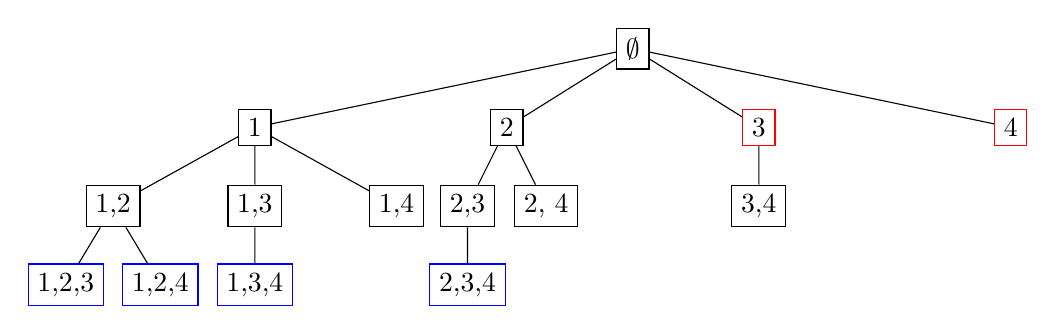
\begin{tikzpicture}
     \node [rectangle,draw]{$\emptyset$} [level distance=10mm,sibling distance=32mm]
     % \node (rect) at (4,2) [draw,thick,minimum width=2cm,minimum height=2cm] {};

    child { node [rectangle,draw]{1} [level distance=10mm ,sibling distance=18mm]
        child {node [rectangle,draw] {1,2} [level distance=10mm ,sibling distance=12mm]
            child {node [rectangle,draw=blue] {1,2,3}
               }
            child {node [rectangle,draw=blue]{1,2,4}}}
        child {node [rectangle,draw] {1,3}
            child {node [rectangle,draw=blue]{1,3,4}}}
        child {node [rectangle,draw] {1,4}}
    }
    child {node [rectangle,draw] {2} [level distance=10mm ,sibling distance=10mm]
        child {node [rectangle,draw] {2,3}
            child {node [rectangle,draw=blue]{2,3,4}}}
        child {node [rectangle,draw]{2, 4}}
    }
    child {node [rectangle,draw=red] {3}
    child {node [rectangle,draw] {3,4}}
    }
    child {node [rectangle,draw=red] {4} 
    }
    ;
    \end{tikzpicture}
\end{center}


\caption{Tree consisting of all element subsets for $n=4$ and $h=3$. Leaves with blue border color represents $h$-element subsets.}
\label{figure:full:tree}
\end{figure}


In the case of the exhaustive approach, we can then traverse the tree starting in the root using the left to right (LTR) preorder traversal, and in each node, we can calculate the OLS fit on $\vec{ X_{J_k} }$ and $\vec{ Y_{J_k} }$. If we are in the level $k = h$, we calculate the fit on the $h$ element subset. This approach is exhaustive, so let us now describe how we can improve efficiency. 

First, it is not necessary to calculate fit on $k$th level of the tree in a case $k < p$ because this would mean that matrix $\vec{ X_{J_k} }$ is not regular. The main improvement can because we can skip parts of the tree (perform pruning) based on the following criteria. Moreover at some point of the traversal we encounter nodes from which we cannot get into the depth $h$ these nodes can also be skipped. On the Figure~\ref{figure:full:tree} these nodes are highlighted with red border color. 

If at any step (at any node) of the tree traversal we calculate the
$\oflts(m_k)$ where $m_{k_i} = 1$ when $k_i \in J_k$ and $m_{k_i} = 0$ and we find out that this value is higher than minimal value found for some $\oflts(m_h)$ thus value of OLS fit on some $h$-element subset, then we can discard all subsets which contain $J_k$. That means we can trim all descendants of the node which represent $J_k$ subset.

We can describe the algorithm as follows:

\begin{enumerate}
    \item Set $RSS^* = \inf$, $m^* = \emptyset$, $\vec{{w}^*} = \emptyset$ 
    \item For each node in LTR preorder traversal calculate $\oflts(m_k)$
    \item If $\oflts(m_k) > RSS^*$, skip all siblings of this node in the traversal.
    \item If $\oflts(m_k) < RSS^* $ and $k = h$, then set $RSS^* = \oflts(m_k)$, $m^*$ so that $m_{k_i} = 1$ when $k_i \in J_k$ and $m_{k_i} = 0$ and $\vec{{w}^*} = \vec{\hat{w}}^{(OLS,\vec{M}_{k}\vec{X}, \vec{M}_{k}\vec{y})}$.
 \item After the traversal return $m^*$ and $\vec{\hat{w}^*}$
\end{enumerate}

Note that during the traversal of the tree, we only need to know the path back to the root. Thus the whole tree does not have to be held in the memory. 

\begin{remark}
If we calculated $\oflts(m_{k})$ than we do not need to calculate $\oflts(m_{k+1})$ from scratch. In Section~\ref{oeamoeammea} we described the way how to update it when a row is added using the matrix inversion any we can apply it here. In Section~\ref{differentcomputation} we described the way of doing this using the matrix decomposition which is another option. 

Moreover, we described that if rows are not extracted and only inserted, then matrix $\vec{Q}$ do not have to be present and only matrix $\vec{R}$ can be updated. We can use this in our favor because we can keep all the decompositions on the path from the root in the memory so we updated the decomposition only when inserting the rows to the matrix $\vec{X}$.  If we use matrix $\vec{\tilde{Z}}$ and $\vec{\tilde{R}}$ we can  (see Remark~\ref{qnotrequiredspeedupremark} ) calculate all the quantities required for the update only using the matrix $\vec{\tilde{R}}$. This means that both versions of updating are possible and both can be done in $\mathcal{O}(p^2)$.
\end{remark}

\subsection{Improvements}
Because the tree is pruned based on the smallest value $RSS^*$, it would be convenient if we were able to obtain small value $RSS^*$ early in the traversal. We can obtain this value by calculating an approximative LTS estimate. This can be done using any probabilistic algorithm described in the previous sections of this chapter. An ideal candidate may be some combined algorithm described in Section~\ref{sectioncombined}. When we find such small value, it is then also convenient to permutate the observations based on its absolute residuals based on this LTS estimate in the decreasing order. That means that during the traversal first $h$-element subset we encounter represents the best known sub-optimal solution given by the approximative algorithm.

Another improvement can be made using the following sorting rule \defterm{sorting rule}: If we are at the level $k$ ( we assume that $k > p$ )
in the node $J_k$ and this node has $s$ siblings indexed as $s_1 \ldots s_s$ then we can change the order of those siblings first by calculating partial increment~\eqref{gamma:plus} for each sibling and consequently ordered them in the descending order from left to right. This means we visit siblings with a lowest partial increment first. Trimming can then be done in the same manner. Moreover, if we calculate $RSS$ in one of those siblings we and realize that $RSS > RSS^*$, then we can on the top of trimming all siblings of this sibling trim also all brothers left to this sibling. That means we can trim parent node $J_k$ because all of his siblings have already been explored or can be trimmed.

% We can see such a procedure at Figure~\ref{figure:sorting:rule}.

% \begin{figure}[h]
% \centering

% \begin{center}
%     \begin{tikzpicture}
%      \node [rectangle,draw]{$\emptyset$} [level distance=10mm,sibling distance=32mm]
%      % \node (rect) at (4,2) [draw,thick,minimum width=2cm,minimum height=2cm] {};

%     child { node [rectangle,draw]{1} [level distance=10mm ,sibling distance=10mm]
%         % child {node [rectangle,draw] {1,2} [level distance=10mm ,sibling distance=12mm]
%         %     child {node [rectangle,draw=blue] {1,2,3}
%         %        }
%         %     child {node [rectangle,draw=blue]{1,2,4}}}
%         % child {node [rectangle,draw] {1,3}
%         %     child {node [rectangle,draw=blue]{1,3,4}}}
%         % child {node [rectangle,draw] {1,4}}
%     }
%     child {node [rectangle,draw] {2} 
%     }
%     child {node [rectangle,draw=red] [level distance=20mm ,sibling distance=50mm] {3}
%         child {node [rectangle,draw] (1) {2,3}}
%         child {node [rectangle,draw] (2) {2, 4}}
%         child {node [rectangle,draw] (5) {2, 4}}
%         child {node [rectangle,draw]{2, 4}}
%     }
%     child {node [rectangle,draw=red] {4} };

%     \node at ($(1)!.5!(2)$) {\ldots};

%     % \draw (1) -- (5);
%     \end{tikzpicture}
% \end{center}


% \caption{Step in the algorithms when due to the sorted siblings node $j_k$ can be trimmed}
% \label{figure:sorting:rule}
% \end{figure}



%%%%%%%%%%%%%%%%%%%%%%%%%%%%%%%%%%%%
%%%%% BSA ALGORITHM  %%%%%%%%%%%%%%%
%%%%%%%%%%%%%%%%%%%%%%%%%%%%%%%%%%%%


\section{BSA algorithm} \label{bsasection}
In this section, we'll introduce another exact algorithm. It has a little different approach than previous algorithms. First of all, build a theoretical basis for this algorithm.



\subsubsection{Domain of OF-LTS}
We introduced two version of OF-LTS. First one is 
$\of^{(LTS,h, n)}(\vec{w}), \vec{w} \in \mathbb{R}^p$ and the second is discrete version 
$\oflts(\vec{m}), \vec{m} \in Q^{(n,h)}$. 
We also know that 
$\minim_{\vec{w} \in \mathbb{R}^p} \of^{(LTS,h, n)}(\vec{w})  =  \minim_{\vec{m} \in Q^{(n,h)}} \oflts(\vec{m})$.

% Let us now extend this relationship.
 (see~\eqref{kloudaodvozeni}) Let us now talk about the non-discrete version and introduce some new feature.

\begin{definition}
    Let $Z \subset \mathbb{R}^p \times  Q^{(n,h)}$ be an relation defined as
    \begin{equation}
        (\vec{w}, \vec{m}) \in Z \Leftrightarrow \sum\limits_{i=1}^h r_{i:n}^2(\vec{w}) = \sum\limits_{i=1}^n m_i r_{i}^2(\vec{w})
    \end{equation}
\end{definition}


$Z$ is not a mapping. To show this we can take simple example so that $r^{2}_{h} = r^{2}_{h+1}$. Then we have for the given $\vec{w}$ two different vectors $\vec{m}$ that are in relation with it.

For that reason, let us define  $\mathcal{U} \subset \mathbb{R}^{p}$ as a maximal set where $Z$ is a mapping. Next we define 
$\mathcal{H} = \mathbb{R}^{p}  \setminus   \mathcal{U}$
as a complement of $\mathcal{U}$.

Let's now describe some properties based on which $\vec{w}$ is in $\mathcal{U}$ or $\mathcal{H}$ set.

\begin{theorem} \label{klouda1}
    $\vec{w} \in \mathcal{U}, \vec{w} \in \mathbb{R}^{p}$ if and only if 
    $r^{2}_{(h:n)}(\vec{w}) < r^{2}_{(h+1:n)}(\vec{w})$
\end{theorem}
\begin{proof}
    As shown in example above. If $r^{2}_{i}(\vec{w}) = r^{2}_{(h:n)}(\vec{w}) = r^{2}_{(h+1:n)}(\vec{w}) = r^{2}_{j}(\vec{w}), i,j \in   \{{1,2,\ldots , n\}} $ then $(\vec{w}, \vec{m_1}) \in Z$ and also $(\vec{w}, \vec{m_2}) \in Z$ where $\vec{m_1}$ has ones at indexes of $h$ smallest residuals and $\vec{m_2}$ has ones at the same indexes except swap $i$th one with $j$th zero.
\end{proof}

\begin{corollary}
    Complement of vectors $\vec{w}$ from Theorem~\ref{klouda1} are vectors such that 
    \begin{equation}
        r^{2}_{(h:n)}(\vec{w}) = r^{2}_{(h+1:n)}(\vec{w})
    \end{equation}
    thus
    \begin{equation}
        \mathcal{H} = \{{ \vec{w} \in \mathbb{R}^{p} | r^{2}_{(h:n)}(\vec{w}) = r^{2}_{(h+1:n)}(\vec{w}) \}}.
    \end{equation}
    That means that for each $\vec{w} \in \mathcal{H}$ there are two different $(\vec{x_i}, y_i)$ and  $(\vec{x_j}, y_j)$ so that
    \begin{equation}
        (y_i - \vec{x_i} \vec{w})^2 = r^{2}_i(\vec{w}) =  r^{2}_{(h:n)}(\vec{w}) = r^{2}_{(h+1:n)}(\vec{w}) =  r^{2}_j(\vec{w}) = (y_j - \vec{x_j} \vec{w})^2.
    \end{equation}

    We can see that 
    \begin{equation}
        (y_i - \vec{x_i} \vec{w})^2 =  (y_j - \vec{x_j} \vec{w})^2 \iff      y_i \pm y_j + (\vec{x_i} \pm \vec{x_j})  \vec{w} = 0
    \end{equation}
\end{corollary}


\begin{assumption} \label{klouda:asump:1}
    For $\vec{X} \in \mathbb{R}^{n \times p}$ let as assume that for all $i,j, \in \{{1,2 \ldots, n \}}$  if $ i \neq j$ then $\vec{x_i} \neq \pm \vec{x_j}$ and $\norm{\vec{x_i}} \neq 0$.
\end{assumption}

If Assumption~\ref{klouda:asump:1} is fulfilled then $ y_i \pm y_j + (\vec{x_i} \pm \vec{x_j})  \vec{w} = 0$ represents a hyperplane. 

It's easy to show that set $\mathcal{U}$ is an open and Lebesgue measure of $\mathcal{H}$  is $0$~\cite{klouda2015exact}. Moreover $\mathcal{H}$ splits $\mathbb{R}^{p}$ into finite number of $m$ open disjoint subsets of $\mathcal{U}$. 

\begin{definition}
    Let's define set of $m \in \mathbb{N}$ sets $\mathcal{U}^{(set)} = \{{ U_i\}}_{i=1}^{m}$ so that
    all $U_i$ are open and connected sets, $U_i$ $U_j$ are disjoined thus $U_i \cap  U_j = \emptyset$, $\cup_{i=1}^{m}    U_i = \mathcal{U}$ and $\cup_{i=1}^{m}    \partial U_i =  \mathcal{H}$.

    We define neighbor sets $U_i, U_j, i \neq j$ so that $ U_i \cap U_j \neq \emptyset$. 

    We also define $M^{(min)}$ set of $m$ vectors $\vec{m} \in Q^{(n,h)}$ so that 
    \begin{equation*}
        M^{(min)} = \{{ \vec{m_1}, \ldots, \vec{m_m} | \vec{m_i} = Z(\vec{w}) \vec{w} \in U_i  \}}.
    \end{equation*}
    where $Z(\vec{w})$ represent unique vector $\vec{m_i}$. That means $Z(\vec{w}) = Z(\vec{w^{\prime}})$ for all $w, w^{\prime} \in U_i$.
\end{definition}

For a better understanding definition above see \missingfigure{p=1 n=5 h=3. visualise all $U_i$ and elements of $\mathcal{H}$}


We say that matrix $\vec{X} \in \mathbb{R}^{n \times p}$ has \defterm{$h$-full} if for all $m \in \qnh$ matrix $\vec{M}\vec{X}$ has rank $p$.

\begin{theorem} \label{minimas:in:relation}
    If the matrix $\vec{X}$ has $h$-full rank then for every local minima at point satisfying weak-necessary condition $\vec{w_{0}}$ of the OF-LTS function, then there exists a vector $\vec{m} \in Q^{(n,h)}$ such that $(\vec{w_{0}}, \vec{m}) \in Z$.
\end{theorem}

Proof can be found in~\cite[Theorem~7]{klouda2015exact}. 

\subsection{ One-dimensional version of the algorithm}

Based on the Theorem~\ref{minimas:in:relation} we can see that
\begin{equation}
    \minim_{\vec{m} \in Q^{(n,h)}} \of^{(OLS,\vec{M}\vec{X}, \vec{M}\vec{Y})} (\vec{w}) =
    \minim_{m \in M^{(min)}} \of^{(OLS,\vec{m^i}\vec{X}, \vec{m^i}\vec{Y})} (\vec{w})
\end{equation}

where $\vec{M} = diag(\vec{m})$, $\vec{m^i} = diag(m)$. Set $M^{(min)}$ is very useful because we can iterate only through this set and not through whole $Q^{(n,h)}$.

Then minimizing objective function $\oflts(\vec{m})$~\eqref{oflts_discrete} can be reformulated as 
\begin{equation} \label{mminqnh}
    \minim_{\vec{m} \in Q^{(n,h)}}  \oflts(\vec{m}) = \minim_{m \in M^{(min)}} \oflts(m)
\end{equation}


That means if we can find all $m \in M^{(min)}$ then minimizing $\oflts$ would be easy.
So how we can find the elements of $M^{(min)}$ set? 

For now, let us assume that we know elements of $\mathcal{H}$.

Because for each $m \in M^{(min)}$ exists at least one $\vec{w} \in \mathcal{H}$ such that $(\vec{w}, \vec{m}) \in Z$ then for given $\vec{w} \in \mathcal{H}$ we can find all $\vec{m}$ by algorithm described by following pseudocode:

\todo{write the pseudocode}
\begin{algorithm}[H]
    \label{find:all:m}
            \KwIn{$\vec{Q} \in \mathbb{R}^{n \times n}, \vec{R} \in \mathbb{R}^{n \times p}, \vec{x_j} \in \mathbb{R}^p, k $}
        \KwOut{ $\vec{Q^{(+)}} \in \mathbb{R}^{n+1 \times n+1}, \vec{R^{(+)}} \in \mathbb{R}^{n+1 \times p}$ }

      \caption{Find all $\vec{m}$}
    %   $\vec{R^{(+)}} \gets \vec{R}~with~appended~last~row~by~\vec{x_j}$\;
    %   $\vec{Q^{(+)}} \gets \vec{Q}~with~appended~last~row~and~last~column~by~zeors$\;
    %   $\vec{Q^{(+)}}_{n+1, n+1} \gets 1$ \tcp*{i.e.  ${Q^{(+)}}$ now has $1$ on the diagonal}


    %   \For{$i \gets n$ \textbf{to} $p$}{
    %     $\vec{Q}(i, n+1) \gets create~Givens~matrix \vec{Q}(i, n+1) \in \mathbb{R}^{n+1 \times n+1}$\;
    %     $\vec{R^{(+)}} \gets   \vec{Q}(i, n+1) \vec{R^{(+)}} $\;
    %     $\vec{Q^{(+)}} \gets \vec{Q^{(+)}} \vec{Q}^T(i, n+1) $\;        
    %     }
      
    % \For{$i \gets n+1$ \textbf{to} $k$}{
    %     $\vec{Q^{(+)}} \gets  \vec{Q^{(+)}} where~we~swap~the~i~row~with~the~i-1~row$
    % }

    \Return{ $\vec{Q^{(+)}}$\,, $\vec{R^{(+)}}$ }\;
\end{algorithm}


Finally we need to find all elements of $\mathcal{H}$. As we know for all elements $\vec{w} \in \mathcal{H}$ $r^{2}_{(h:n)}(\vec{w}) = r^{2}_{(h+1:n)}(\vec{w})$. So if we find all $\vec{w}$ that solve this, then we found $\mathcal{H}$. The problem is that residuals are sorted. To overcome this issue by finding some candidates which would possible be equal $(h:n)$th and $(h+1:n)$th squared residuals. In~\cite{klouda2015exact} we are provided necessary condition for such a candidates.

\begin{definition}
    If $\vec{w} \in \mathcal{H}$ then there exists $i,j, i \neq j$ so that
     $r^{2}_i(\vec{w}) = r^{2}_j(\vec{w})$. We denote set $H$ containing $\vec{w}$ satisfying this necessary condition, thus

    \begin{equation}
        H = \{{ \vec{w} \in \mathbb{R}^p | r^{2}_i(\vec{w}) = r^{2}_j(\vec{w}), i \neq j  \}}.   
    \end{equation}
     
\end{definition}

Note that $|H| \leq 2 \choose{n}{p+1}$. So in  the case of the one dimensional case $|H| \leq 2 \choose{n}{2} = n(n-1)$.

Finding all elements of $H$ is then equal for for solving $\choose{n}{p+1}$ equations. Moreover, because equations are quadratic, we can have up to two solutions for each equation.

So idea of the whole algorithm is to find all elements of $H$ (by solving quadratic equations), consequently finding which of them are part of $\mathcal{H}$ (by ordering squared residuals and checking if $r^{2}_{(h:n)}(\vec{w}) = r^{2}_{(h+1:n)}(\vec{w}$) and finally for each $\vec{w} \in \mathcal{H}$ find $\vec{m}$ that are in relation. All of those $\vec{m}$ vectors form $M^{(min)}$ set. Finally we can use $\vec{m} \in M^{(min)}$ for minimizing $\oflts(\vec{m})$ by the terms of~\eqref{mminqnh}. The whole algorithm, which authors call Border Scanning Algorithm (BSA) is described by the following pseudocode:

\todo{write the pseudocode}
\begin{algorithm}[H]
    \label{alg:border:scanning:bsa:onedim}
            \KwIn{$\vec{Q} \in \mathbb{R}^{n \times n}, \vec{R} \in \mathbb{R}^{n \times p}, \vec{x_j} \in \mathbb{R}^p, k $}
        \KwOut{ $\vec{Q^{(+)}} \in \mathbb{R}^{n+1 \times n+1}, \vec{R^{(+)}} \in \mathbb{R}^{n+1 \times p}$ }

      \caption{BSA}
    %   $\vec{R^{(+)}} \gets \vec{R}~with~appended~last~row~by~\vec{x_j}$\;
    %   $\vec{Q^{(+)}} \gets \vec{Q}~with~appended~last~row~and~last~column~by~zeors$\;
    %   $\vec{Q^{(+)}}_{n+1, n+1} \gets 1$ \tcp*{i.e.  ${Q^{(+)}}$ now has $1$ on the diagonal}


    %   \For{$i \gets n$ \textbf{to} $p$}{
    %     $\vec{Q}(i, n+1) \gets create~Givens~matrix \vec{Q}(i, n+1) \in \mathbb{R}^{n+1 \times n+1}$\;
    %     $\vec{R^{(+)}} \gets   \vec{Q}(i, n+1) \vec{R^{(+)}} $\;
    %     $\vec{Q^{(+)}} \gets \vec{Q^{(+)}} \vec{Q}^T(i, n+1) $\;        
    %     }
      
    % \For{$i \gets n+1$ \textbf{to} $k$}{
    %     $\vec{Q^{(+)}} \gets  \vec{Q^{(+)}} where~we~swap~the~i~row~with~the~i-1~row$
    % }

    \Return{ $\vec{Q^{(+)}}$\,, $\vec{R^{(+)}}$ }\;
\end{algorithm}


\subsection{Multidimensional BSA}

If we would like to scale the algorithm into the higher dimension, we have to face one major complication. The algorithm finds all elements of $H$ and $\mathcal{H}$. This is possible in one dimension, but because $\mathcal{H}$ forms a hyperplane, then for higher dimensions is infinite.

Authors then propose to find finite set $mathcal{H}_p$ such that 
\begin{equation} \label{hp:set:condition}
    \forall \vec{m} \in M^{(min)} \exists \vec{w} \in \mathcal{H}_p : (\vec{w},\vec{m}) \in Z
\end{equation}

and also finite set $H_p$, so that $mathcal{H}_p \subset H_p \subset H$. We can see that for $p=1$ we need only one equation so the solution has dimension $0$. If we would like to have some solution with dimension equal to $0$ for $p > 1$ we need system of $p$ equations. Moreover this system of equations have to be independent. So we can consider system of $p$ equations of type $ r^{2}_i(\vec{w}) = r^{2}_j(\vec{w})$

\begin{align} 
    r^{2}_{i_1}(\vec{w}) &= r^{2}_{i_2}(\vec{w}) \label{p:plus:one:equations}   \\
    r^{2}_{i_2}(\vec{w}) &= r^{2}_{i_3}(\vec{w}) \nonumber  \\
    \vdots \ \ \  & \ \ \ \  \ \vdots  \nonumber \\ 
    r^{2}_{i_p}(\vec{w}) &=  r^{2}_{i_{p+1}}(\vec{w}) \nonumber 
\end{align}

where $i_1, i_2 \ldots i_{p+1}$  is $(p+1)$-element subset of ${1, 2, \ldots n}$.


System of those quadratic equations can be rewritten as 
Because this is a system of quadratic equations, we can have up to $2^p$ solutions.

Moreover total number of $(p+1)$-element subsets out of $n$ is $\binom{n}{p+1}$.
This means that the total number of solutions can be up to $\binom{n}{p+1} 2^p$. 
We denote set of all these solutions $H_p$.

So if set $H_p$ satisfies~\eqref{hp:set:condition} then it can be used for finding $\mathcal{H}_p$ subset, thus we would be able to use this set for the multidimensional version of the algorithm.

Let $\circ \in {+, -}$ be either operation $+$ or $-$. Then system of quadratic equations~\eqref{p:plus:one:equations} is equivalent to $2^p$ linear systems

\begin{align} 
    (\vec{x}_{i_1} \circ_1 \vec {x}_{i_2} )^T \vec{w} &= y_{i_1} \circ_1 y_{i_2} \label{p:plus:one:equations:linear}   \\
    \vdots \ \ \  & \ \ \ \  \ \vdots  \nonumber \\ 
    (\vec{x}_{i_p} \circ_p \vec {x}_{i_{p+1}} )^T \vec{w} &= y_{i_p} \circ_p y_{i_{p+1}}. \nonumber 
\end{align}

Moreover~\eqref{p:plus:one:equations:linear} is equivalent to the set of equations


\begin{align} 
    (\vec{x}_{i_1} \circ_1 \vec {x}_{i_2} )^T \vec{w} &= y_{i_1} \circ_1 y_{i_2} \label{p:plus:one:equations:linear:simple}   \\
    \vdots \ \ \  & \ \ \ \  \ \vdots  \nonumber \\ 
    (\vec{x}_{i_1} \circ_p \vec {x}_{i_{p+1}} )^T \vec{w} &= y_{i_1} \circ_p y_{i_{p+1}}. \nonumber 
\end{align}
Elements of set $\mathcal{H}_p$ then satisfies $r_{i_1^2}(\vec{w}) = r_{(h:n))}(\vec{w}) = r_{(h+1:n))}(\vec{w})$.


Set $H_p$ was proven to be suitable for finding $\mathcal{H}_p$ in~\cite{klouda2015exact} thus that set $\mathcal{H}_p$ satisfies~\eqref{hp:set:condition} if following assumptions are satisfied (we already assume that Assumption~\ref{klouda:asump:1} holds). First is that for all $\vec{w}$ $r_{(h:n))}(\vec{w}) > 0$, second , for all 
$(\circ_1,\circ_2 \ldots,  \circ_{n-1}) \in \times^n_{i=1} {+, -}$ the matrix system of $n-1$ equations

\begin{align} 
    (\vec{x}_{i_1} \circ_1 \vec {x}_{i_2} )^T \vec{w} &= y_{i_1} \circ_1 y_{i_2} \label{p:plus:one:equations:linear:simple:to:n}   \\
    \vdots \ \ \  & \ \ \ \  \ \vdots  \nonumber \\ 
    (\vec{x}_{i_1} \circ_{n-1} \vec {x}_{i_{n}} )^T \vec{w} &= y_{i_1} \circ_p y_{i_{n}}. \nonumber.
\end{align}
The seconds assumption prevents the set $\mathcal{H}_p$ to be empty thus the case where all systems~\eqref{p:plus:one:equations:linear:simple} are dependent. 

This assumption can cause problem because when we assume model with the intercept, thus for all rows $\vec{x_i}$ of matrix $\vec{X}$ is $x_{i1} = 1$ then in the case  $\circ_1,\circ_2 \ldots,  \circ_{n-1} = -$, first column of matrix $\vec{X}$ only contains zeroes. We can modify this assumption so that instead of using $(\circ_1,\circ_2 \ldots,  \circ_{n-1}) \in \times^n_{i=1} {+, -}$ we use only $(\circ_1,\circ_2 \ldots,  \circ_{n-1}) \in \times^n_{i=1} {+, -} \setminus {(-, \ldots, -)}$~\cite{klouda2015exact}. 

Given that we now know that set $H_p$ and $\mathcal{H}_p$ are suitable for our algorithm and we also know how to calculate them, so let us describe the multidimensional version of the algorithm.

\todo{write the pseudocode}

Let us now describe the time complexity of this algorithm. 

\todo{write the time complexity}